\documentclass{beamer}
\usepackage[utf8]{inputenc}
\usepackage[T1]{fontenc}
\usepackage{fancyvrb}
\title{Deep Learning on the IMDB Dataset}
\date{WASP Deep Learning}
\author[Agents 47]{The Hitmen --- Agents 47}

%\usepackage{enumitem}

\usepackage{pgfplots}
\pgfplotsset{compat=1.8}
\usepackage{pgfplotstable}
\usepgfplotslibrary{groupplots}

\newlength\figureheight
\newlength\figurewidth

\usetheme{wasp}

\graphicspath{{./graphics/}}

\usepackage{lipsum}
\newcommand\blfootnote[1]{%
	\begingroup
	\renewcommand\thefootnote{}\footnote{#1}%
	\addtocounter{footnote}{-1}%
	\endgroup
}

\begin{document}

\begin{frame}
  \titlepage
\end{frame}


\begin{frame}{Convnets}{Convolutional Neural Networks}

  \begin{itemize}

  \item[Training] Using all data, we reached the best result after around 1 or 2
    epochs to around 93.5 \%. By using less, say 20 \% of the data, training
    improved for up to 4 epochs, but the validation results were considerably
    worse (73 \%). Note however that training with less data is considerably
    faster.

  \item[Batch] Smaller batches train slightly faster, but doesn't otherwise
    affect validation results much (Got 94.1 \% with batch size 64). Too big
    batches may however consume too much memory for efficient training.

  \end{itemize}

\end{frame}

\begin{frame}
  \begin{itemize}

  \item[Choices] Increasing these values can add a significant amount of data to
    the model, and thus \textbf{might} improve the result (93.7 \%), but will
    also take longer to train. Reducing it barely changs the result. (93.1 \%).

  \item[Dropout] 20\% dropout helps slightly: 94.7 \%.  40\% dropout helps a bit
    more: 95.5 \%. Even higher (80 \%) didn't improve the final result, but did
    make the learning process improve for all 10 epochs.

  \item[Archs] Krohn's architecture seems to perform slightly better, but takes
    a little longer to train than Chollet's. Comparing this with a network
    architecture with only dense layers (~88 \%), convolutional architectures
    seem superior.

  \end{itemize}

\end{frame}

\iffalse
\begin{frame}{Convnets}{Training History}

  \begin{columns}
    \begin{column}{0.5\textwidth}
      \begin{figure}[ht]
        \centering
        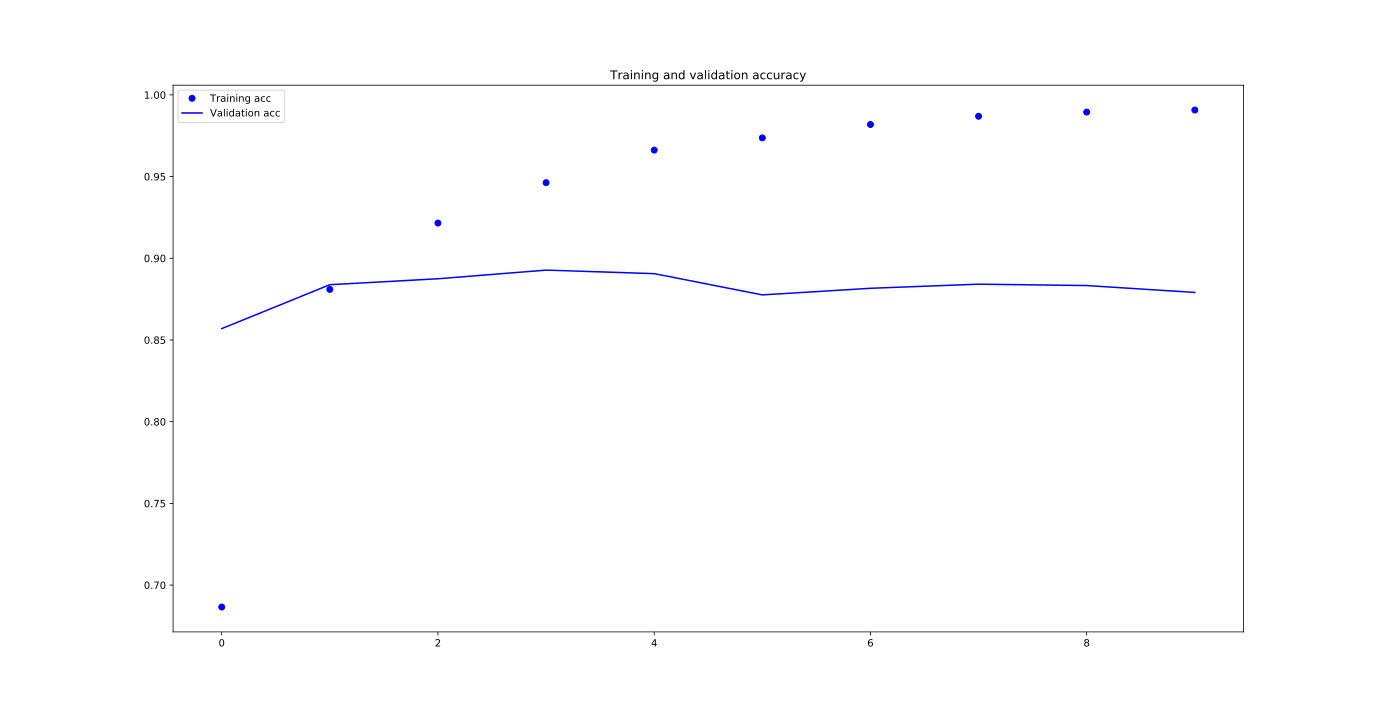
\includegraphics[width=1.2\textwidth]{convnet_training}
      \end{figure}

    \end{column}
    \begin{column}{0.5\textwidth}
      \begin{figure}[ht]
        \centering
        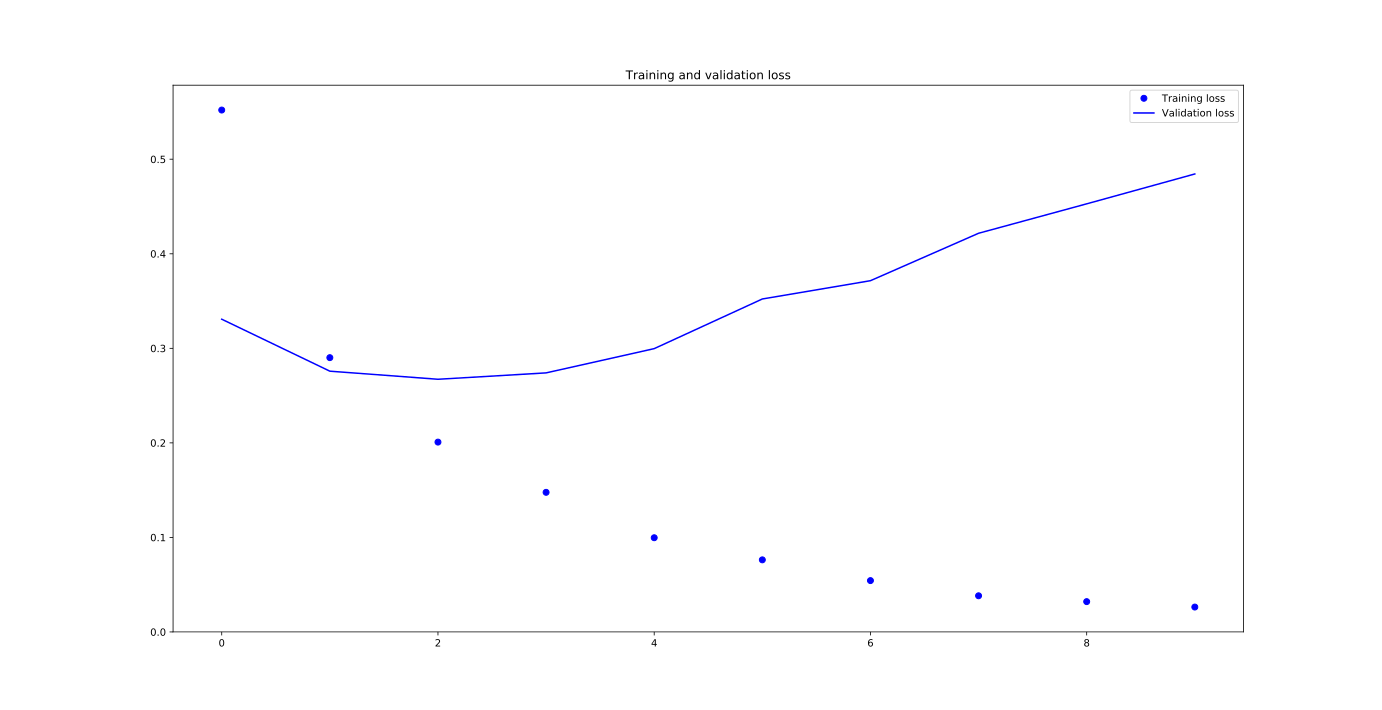
\includegraphics[width=1.2\textwidth]{convnet_loss}
      \end{figure}

    \end{column}
  \end{columns}

\end{frame}

\begin{frame}{Convnets}{Classification Confidence}

  \begin{figure}[ht]
    \centering
    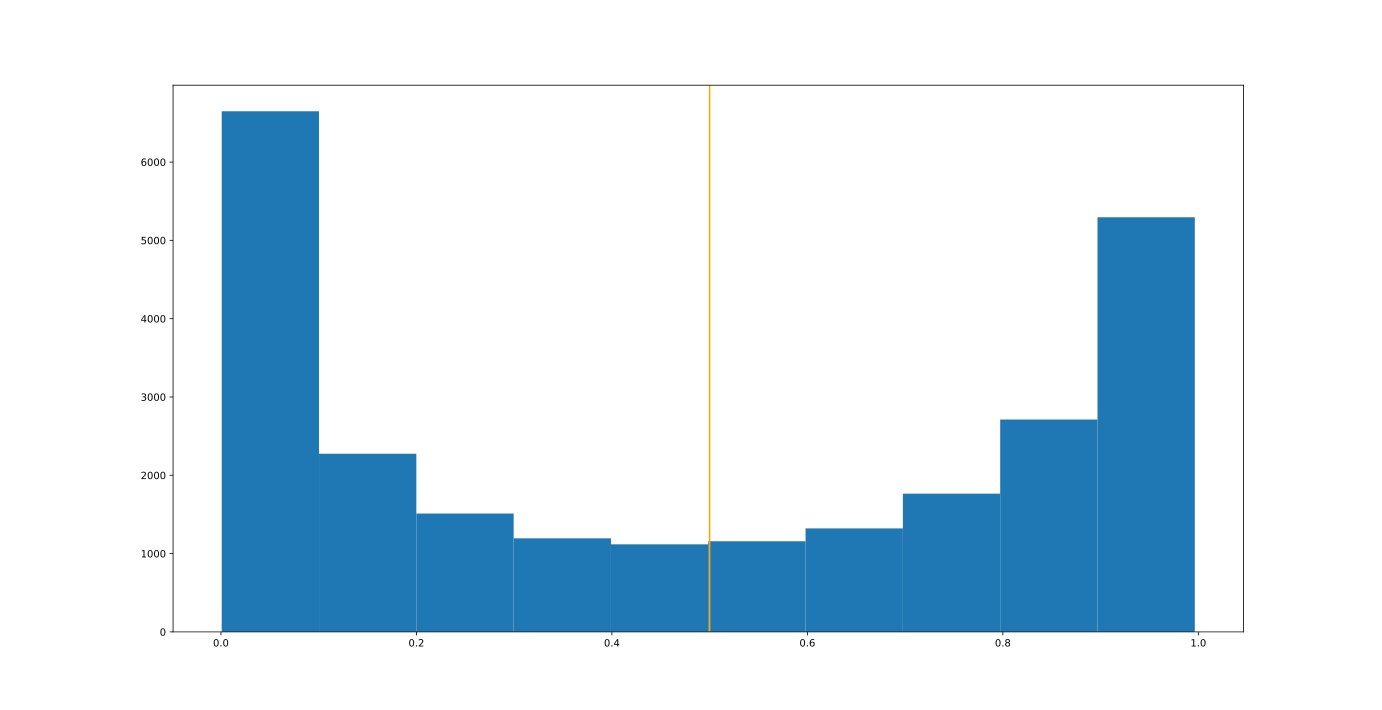
\includegraphics[width=0.7\textwidth]{convnet_histogram}
  \end{figure}

\end{frame}
\fi


\begin{frame}{Convnets}{Why Convolutions for NLP?}

  \begin{itemize}

  \item Intuitively, a 1D convolution would look both forwards and backwards in
    a sentence, mimicking how the natural language refers to earlier or coming
    words.

  \item Training for more than 2 or 3 epochs doesn't appear to be beneficial for
    classification of this data. This does however depend quite a lot on
    hyper-parameter choices.

  \item Best validation score: 95.96 \%.

  \end{itemize}

\end{frame}



\begin{frame}{RNN}{Recurrent Neural Networks}

	Output of the layer is fed back into the layer, which can be seen as a recursion over a time series.

	\begin{figure}
		\centering
		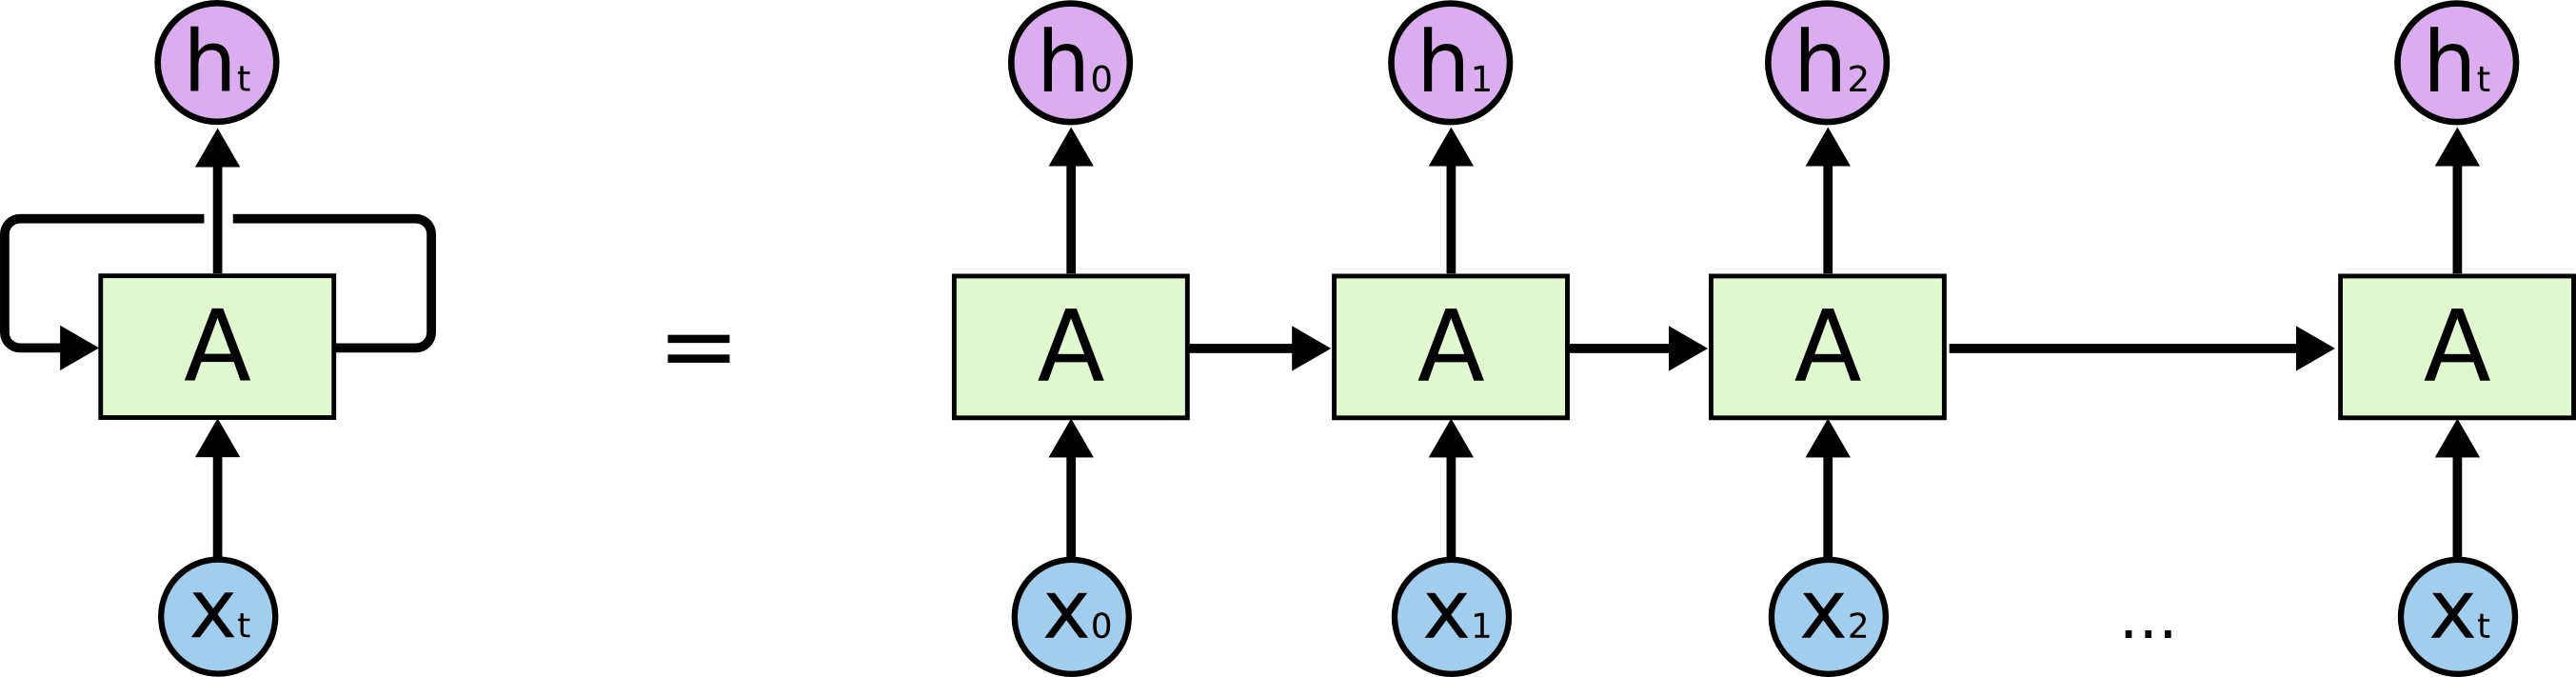
\includegraphics[width=0.7\linewidth]{graphics/RNN-unrolled.png}
	\end{figure}

	Testing the impact of stacking layers, 4 models in total are trained. Model 1 contains 1 32-sized RNN layer with 0.2 dropout, Model 2 contains 2 such layers and so on. This is then trained for 5 epochs with 128 batch size. 


\blfootnote{\tiny Image courtesy of Christopher Olah, \url{http://colah.github.io/posts/2015-08-Understanding-LSTMs/}}
  
\end{frame}

\begin{frame}{RNN}{Recurrent Neural Networks}
	\begin{figure}
	\centering

	\setlength\figureheight{3cm}
	\setlength\figurewidth{0.5\linewidth}
	
	% This file was created by matplotlib2tikz v0.6.18.
\begin{tikzpicture}

\begin{groupplot}[group style={group size=2 by 2}]
\nextgroupplot[
height=\figureheight,
tick align=outside,
tick pos=left,
title={Model 1},
width=\figurewidth,
x grid style={lightgray!92.02614379084967!black},
xmin=-0.2, xmax=4.2,
y grid style={lightgray!92.02614379084967!black},
ymin=0.5, ymax=1,
xticklabels={,,,,}
]
\addplot [semithick, blue, mark=*, mark size=3, mark options={solid}, only marks, forget plot]
table [row sep=\\]{%
0	0.605879999961853 \\
1	0.775800000038147 \\
2	0.865720000019073 \\
3	0.912959999980926 \\
4	0.939960000019074 \\
};
\addplot [semithick, blue, forget plot]
table [row sep=\\]{%
0	0.762640000038147 \\
1	0.773159999980927 \\
2	0.842439999980927 \\
3	0.828439999961853 \\
4	0.852039999980926 \\
};
\nextgroupplot[
height=\figureheight,
tick align=outside,
tick pos=left,
title={Model 2},
width=\figurewidth,
x grid style={lightgray!92.02614379084967!black},
xmin=-0.2, xmax=4.2,
y grid style={lightgray!92.02614379084967!black},
ymin=0.5, ymax=1,
xticklabels={,,,,}
]
\addplot [semithick, blue, mark=*, mark size=3, mark options={solid}, only marks, forget plot]
table [row sep=\\]{%
0	0.587199999961853 \\
1	0.854319999961853 \\
2	0.872839999961853 \\
3	0.912079999980926 \\
4	0.942880000019073 \\
};
\addplot [semithick, blue, forget plot]
table [row sep=\\]{%
0	0.81604 \\
1	0.8648 \\
2	0.844160000038147 \\
3	0.849200000019073 \\
4	0.849999999961853 \\
};
\nextgroupplot[
height=\figureheight,
tick align=outside,
tick pos=left,
title={Model 3},
width=\figurewidth,
x grid style={lightgray!92.02614379084967!black},
xmin=-0.2, xmax=4.2,
y grid style={lightgray!92.02614379084967!black},
ymin=0.5, ymax=1
]
\addplot [semithick, blue, mark=*, mark size=3, mark options={solid}, only marks, forget plot]
table [row sep=\\]{%
0	0.522080000019074 \\
1	0.773879999961853 \\
2	0.882079999961853 \\
3	0.926399999961853 \\
4	0.956040000019074 \\
};
\addplot [semithick, blue, forget plot]
table [row sep=\\]{%
0	0.582559999961853 \\
1	0.821520000019073 \\
2	0.816400000019074 \\
3	0.81756 \\
4	0.840599999980926 \\
};
\nextgroupplot[
height=\figureheight,
tick align=outside,
tick pos=left,
title={Model 4},
width=\figurewidth,
x grid style={lightgray!92.02614379084967!black},
xmin=-0.2, xmax=4.2,
y grid style={lightgray!92.02614379084967!black},
ymin=0.5, ymax=1
]
\addplot [semithick, blue, mark=*, mark size=3, mark options={solid}, only marks, forget plot]
table [row sep=\\]{%
0	0.498879999980927 \\
1	0.50836 \\
2	0.601960000019073 \\
3	0.791760000019074 \\
4	0.869559999961853 \\
};
\addplot [semithick, blue, forget plot]
table [row sep=\\]{%
0	0.499999999980927 \\
1	0.525439999990463 \\
2	0.770719999961853 \\
3	0.824199999961853 \\
4	0.820239999961853 \\
};
\end{groupplot}

\end{tikzpicture}
	\caption{Training (circle) vs Validation (line) accuracy.} 
	\end{figure}
\end{frame}

\begin{frame}{RNN}{Recurrent Neural Networks}
	
	\noindent
	\begin{minipage}{0.45\textwidth}%
		 The different models obtain a ROC value of 
		 \begin{itemize}%[noitemsep,topsep=0pt,parsep=0pt,partopsep=0pt]
		 	\item Model 1: 86.34
		 	\item Model 2: 93.49
		 	\item Model 3: 66.09
		 	\item Model 4: 52.38
		 \end{itemize}
	 	Considering the histograms as well, it can be concluded that adding additional layers \emph{can} improve performance but also increases the risk of not converging as seen in Model 3 and 4.
	\end{minipage} \hfill
	\begin{minipage}{0.45\textwidth}%
		\begin{figure}
			\centering
			
			\setlength\figureheight{3cm}
			\setlength\figurewidth{0.5\linewidth}
			
			% This file was created by matplotlib2tikz v0.6.18.
\begin{tikzpicture}

\definecolor{color1}{rgb}{1,0.647058823529412,0}
\definecolor{color0}{rgb}{0.12156862745098,0.466666666666667,0.705882352941177}

\begin{groupplot}[group style={group size=2 by 2}]
\nextgroupplot[
height=\figureheight,
tick align=outside,
tick pos=left,
title={Model 1},
width=\figurewidth,
x grid style={lightgray!92.02614379084967!black},
xmin=0, xmax=1,
y grid style={lightgray!92.02614379084967!black},
ymin=0, ymax=596.4,
xticklabels={,,,,}
]
\draw[fill=color0,draw opacity=0] (axis cs:0.0138896042481065,0) rectangle (axis cs:0.0236279208492488,56);
\draw[fill=color0,draw opacity=0] (axis cs:0.0236279208492488,0) rectangle (axis cs:0.0333662374503911,147);
\draw[fill=color0,draw opacity=0] (axis cs:0.0333662374503911,0) rectangle (axis cs:0.0431045540515333,181);
\draw[fill=color0,draw opacity=0] (axis cs:0.0431045540515333,0) rectangle (axis cs:0.0528428706526756,276);
\draw[fill=color0,draw opacity=0] (axis cs:0.0528428706526756,0) rectangle (axis cs:0.0625811872538179,346);
\draw[fill=color0,draw opacity=0] (axis cs:0.0625811872538179,0) rectangle (axis cs:0.0723195038549602,385);
\draw[fill=color0,draw opacity=0] (axis cs:0.0723195038549602,0) rectangle (axis cs:0.0820578204561025,384);
\draw[fill=color0,draw opacity=0] (axis cs:0.0820578204561025,0) rectangle (axis cs:0.0917961370572448,386);
\draw[fill=color0,draw opacity=0] (axis cs:0.0917961370572448,0) rectangle (axis cs:0.101534453658387,382);
\draw[fill=color0,draw opacity=0] (axis cs:0.101534453658387,0) rectangle (axis cs:0.111272770259529,418);
\draw[fill=color0,draw opacity=0] (axis cs:0.111272770259529,0) rectangle (axis cs:0.121011086860672,460);
\draw[fill=color0,draw opacity=0] (axis cs:0.121011086860672,0) rectangle (axis cs:0.130749403461814,470);
\draw[fill=color0,draw opacity=0] (axis cs:0.130749403461814,0) rectangle (axis cs:0.140487720062956,522);
\draw[fill=color0,draw opacity=0] (axis cs:0.140487720062956,0) rectangle (axis cs:0.150226036664098,531);
\draw[fill=color0,draw opacity=0] (axis cs:0.150226036664099,0) rectangle (axis cs:0.159964353265241,542);
\draw[fill=color0,draw opacity=0] (axis cs:0.159964353265241,0) rectangle (axis cs:0.169702669866383,568);
\draw[fill=color0,draw opacity=0] (axis cs:0.169702669866383,0) rectangle (axis cs:0.179440986467525,563);
\draw[fill=color0,draw opacity=0] (axis cs:0.179440986467525,0) rectangle (axis cs:0.189179303068668,530);
\draw[fill=color0,draw opacity=0] (axis cs:0.189179303068668,0) rectangle (axis cs:0.19891761966981,498);
\draw[fill=color0,draw opacity=0] (axis cs:0.19891761966981,0) rectangle (axis cs:0.208655936270952,439);
\draw[fill=color0,draw opacity=0] (axis cs:0.208655936270952,0) rectangle (axis cs:0.218394252872094,469);
\draw[fill=color0,draw opacity=0] (axis cs:0.218394252872095,0) rectangle (axis cs:0.228132569473237,483);
\draw[fill=color0,draw opacity=0] (axis cs:0.228132569473237,0) rectangle (axis cs:0.237870886074379,444);
\draw[fill=color0,draw opacity=0] (axis cs:0.237870886074379,0) rectangle (axis cs:0.247609202675521,374);
\draw[fill=color0,draw opacity=0] (axis cs:0.247609202675521,0) rectangle (axis cs:0.257347519276664,368);
\draw[fill=color0,draw opacity=0] (axis cs:0.257347519276664,0) rectangle (axis cs:0.267085835877806,341);
\draw[fill=color0,draw opacity=0] (axis cs:0.267085835877806,0) rectangle (axis cs:0.276824152478948,353);
\draw[fill=color0,draw opacity=0] (axis cs:0.276824152478948,0) rectangle (axis cs:0.286562469080091,322);
\draw[fill=color0,draw opacity=0] (axis cs:0.286562469080091,0) rectangle (axis cs:0.296300785681233,334);
\draw[fill=color0,draw opacity=0] (axis cs:0.296300785681233,0) rectangle (axis cs:0.306039102282375,308);
\draw[fill=color0,draw opacity=0] (axis cs:0.306039102282375,0) rectangle (axis cs:0.315777418883517,300);
\draw[fill=color0,draw opacity=0] (axis cs:0.315777418883517,0) rectangle (axis cs:0.32551573548466,248);
\draw[fill=color0,draw opacity=0] (axis cs:0.32551573548466,0) rectangle (axis cs:0.335254052085802,247);
\draw[fill=color0,draw opacity=0] (axis cs:0.335254052085802,0) rectangle (axis cs:0.344992368686944,263);
\draw[fill=color0,draw opacity=0] (axis cs:0.344992368686944,0) rectangle (axis cs:0.354730685288087,232);
\draw[fill=color0,draw opacity=0] (axis cs:0.354730685288087,0) rectangle (axis cs:0.364469001889229,204);
\draw[fill=color0,draw opacity=0] (axis cs:0.364469001889229,0) rectangle (axis cs:0.374207318490371,216);
\draw[fill=color0,draw opacity=0] (axis cs:0.374207318490371,0) rectangle (axis cs:0.383945635091513,200);
\draw[fill=color0,draw opacity=0] (axis cs:0.383945635091513,0) rectangle (axis cs:0.393683951692656,202);
\draw[fill=color0,draw opacity=0] (axis cs:0.393683951692656,0) rectangle (axis cs:0.403422268293798,226);
\draw[fill=color0,draw opacity=0] (axis cs:0.403422268293798,0) rectangle (axis cs:0.41316058489494,195);
\draw[fill=color0,draw opacity=0] (axis cs:0.41316058489494,0) rectangle (axis cs:0.422898901496083,173);
\draw[fill=color0,draw opacity=0] (axis cs:0.422898901496083,0) rectangle (axis cs:0.432637218097225,169);
\draw[fill=color0,draw opacity=0] (axis cs:0.432637218097225,0) rectangle (axis cs:0.442375534698367,171);
\draw[fill=color0,draw opacity=0] (axis cs:0.442375534698367,0) rectangle (axis cs:0.452113851299509,178);
\draw[fill=color0,draw opacity=0] (axis cs:0.452113851299509,0) rectangle (axis cs:0.461852167900652,170);
\draw[fill=color0,draw opacity=0] (axis cs:0.461852167900652,0) rectangle (axis cs:0.471590484501794,151);
\draw[fill=color0,draw opacity=0] (axis cs:0.471590484501794,0) rectangle (axis cs:0.481328801102936,173);
\draw[fill=color0,draw opacity=0] (axis cs:0.481328801102936,0) rectangle (axis cs:0.491067117704079,149);
\draw[fill=color0,draw opacity=0] (axis cs:0.491067117704079,0) rectangle (axis cs:0.500805434305221,129);
\draw[fill=color0,draw opacity=0] (axis cs:0.500805434305221,0) rectangle (axis cs:0.510543750906363,161);
\draw[fill=color0,draw opacity=0] (axis cs:0.510543750906363,0) rectangle (axis cs:0.520282067507505,154);
\draw[fill=color0,draw opacity=0] (axis cs:0.520282067507505,0) rectangle (axis cs:0.530020384108648,158);
\draw[fill=color0,draw opacity=0] (axis cs:0.530020384108648,0) rectangle (axis cs:0.53975870070979,160);
\draw[fill=color0,draw opacity=0] (axis cs:0.53975870070979,0) rectangle (axis cs:0.549497017310932,144);
\draw[fill=color0,draw opacity=0] (axis cs:0.549497017310932,0) rectangle (axis cs:0.559235333912075,154);
\draw[fill=color0,draw opacity=0] (axis cs:0.559235333912075,0) rectangle (axis cs:0.568973650513217,165);
\draw[fill=color0,draw opacity=0] (axis cs:0.568973650513217,0) rectangle (axis cs:0.578711967114359,144);
\draw[fill=color0,draw opacity=0] (axis cs:0.578711967114359,0) rectangle (axis cs:0.588450283715502,143);
\draw[fill=color0,draw opacity=0] (axis cs:0.588450283715501,0) rectangle (axis cs:0.598188600316644,148);
\draw[fill=color0,draw opacity=0] (axis cs:0.598188600316644,0) rectangle (axis cs:0.607926916917786,150);
\draw[fill=color0,draw opacity=0] (axis cs:0.607926916917786,0) rectangle (axis cs:0.617665233518928,148);
\draw[fill=color0,draw opacity=0] (axis cs:0.617665233518928,0) rectangle (axis cs:0.627403550120071,113);
\draw[fill=color0,draw opacity=0] (axis cs:0.627403550120071,0) rectangle (axis cs:0.637141866721213,158);
\draw[fill=color0,draw opacity=0] (axis cs:0.637141866721213,0) rectangle (axis cs:0.646880183322355,154);
\draw[fill=color0,draw opacity=0] (axis cs:0.646880183322355,0) rectangle (axis cs:0.656618499923497,147);
\draw[fill=color0,draw opacity=0] (axis cs:0.656618499923497,0) rectangle (axis cs:0.66635681652464,155);
\draw[fill=color0,draw opacity=0] (axis cs:0.66635681652464,0) rectangle (axis cs:0.676095133125782,169);
\draw[fill=color0,draw opacity=0] (axis cs:0.676095133125782,0) rectangle (axis cs:0.685833449726924,164);
\draw[fill=color0,draw opacity=0] (axis cs:0.685833449726924,0) rectangle (axis cs:0.695571766328067,166);
\draw[fill=color0,draw opacity=0] (axis cs:0.695571766328067,0) rectangle (axis cs:0.705310082929209,145);
\draw[fill=color0,draw opacity=0] (axis cs:0.705310082929209,0) rectangle (axis cs:0.715048399530351,170);
\draw[fill=color0,draw opacity=0] (axis cs:0.715048399530351,0) rectangle (axis cs:0.724786716131493,212);
\draw[fill=color0,draw opacity=0] (axis cs:0.724786716131493,0) rectangle (axis cs:0.734525032732636,183);
\draw[fill=color0,draw opacity=0] (axis cs:0.734525032732636,0) rectangle (axis cs:0.744263349333778,191);
\draw[fill=color0,draw opacity=0] (axis cs:0.744263349333778,0) rectangle (axis cs:0.75400166593492,179);
\draw[fill=color0,draw opacity=0] (axis cs:0.75400166593492,0) rectangle (axis cs:0.763739982536063,178);
\draw[fill=color0,draw opacity=0] (axis cs:0.763739982536063,0) rectangle (axis cs:0.773478299137205,216);
\draw[fill=color0,draw opacity=0] (axis cs:0.773478299137205,0) rectangle (axis cs:0.783216615738347,223);
\draw[fill=color0,draw opacity=0] (axis cs:0.783216615738347,0) rectangle (axis cs:0.792954932339489,254);
\draw[fill=color0,draw opacity=0] (axis cs:0.79295493233949,0) rectangle (axis cs:0.802693248940632,218);
\draw[fill=color0,draw opacity=0] (axis cs:0.802693248940632,0) rectangle (axis cs:0.812431565541774,226);
\draw[fill=color0,draw opacity=0] (axis cs:0.812431565541774,0) rectangle (axis cs:0.822169882142916,246);
\draw[fill=color0,draw opacity=0] (axis cs:0.822169882142916,0) rectangle (axis cs:0.831908198744059,214);
\draw[fill=color0,draw opacity=0] (axis cs:0.831908198744059,0) rectangle (axis cs:0.841646515345201,254);
\draw[fill=color0,draw opacity=0] (axis cs:0.841646515345201,0) rectangle (axis cs:0.851384831946343,216);
\draw[fill=color0,draw opacity=0] (axis cs:0.851384831946343,0) rectangle (axis cs:0.861123148547486,273);
\draw[fill=color0,draw opacity=0] (axis cs:0.861123148547486,0) rectangle (axis cs:0.870861465148628,255);
\draw[fill=color0,draw opacity=0] (axis cs:0.870861465148628,0) rectangle (axis cs:0.88059978174977,258);
\draw[fill=color0,draw opacity=0] (axis cs:0.88059978174977,0) rectangle (axis cs:0.890338098350912,252);
\draw[fill=color0,draw opacity=0] (axis cs:0.890338098350912,0) rectangle (axis cs:0.900076414952055,248);
\draw[fill=color0,draw opacity=0] (axis cs:0.900076414952055,0) rectangle (axis cs:0.909814731553197,232);
\draw[fill=color0,draw opacity=0] (axis cs:0.909814731553197,0) rectangle (axis cs:0.919553048154339,238);
\draw[fill=color0,draw opacity=0] (axis cs:0.919553048154339,0) rectangle (axis cs:0.929291364755481,235);
\draw[fill=color0,draw opacity=0] (axis cs:0.929291364755481,0) rectangle (axis cs:0.939029681356624,184);
\draw[fill=color0,draw opacity=0] (axis cs:0.939029681356624,0) rectangle (axis cs:0.948767997957766,148);
\draw[fill=color0,draw opacity=0] (axis cs:0.948767997957766,0) rectangle (axis cs:0.958506314558908,138);
\draw[fill=color0,draw opacity=0] (axis cs:0.958506314558908,0) rectangle (axis cs:0.968244631160051,158);
\draw[fill=color0,draw opacity=0] (axis cs:0.968244631160051,0) rectangle (axis cs:0.977982947761193,86);
\draw[fill=color0,draw opacity=0] (axis cs:0.977982947761193,0) rectangle (axis cs:0.987721264362335,39);
\addplot [semithick, color1, forget plot]
table [row sep=\\]{%
0.5	0 \\
0.5	1 \\
};
\nextgroupplot[
height=\figureheight,
tick align=outside,
tick pos=left,
title={Model 2},
width=\figurewidth,
x grid style={lightgray!92.02614379084967!black},
xmin=0, xmax=1,
y grid style={lightgray!92.02614379084967!black},
ymin=0, ymax=1407,
xticklabels={,,,,}
]
\draw[fill=color0,draw opacity=0] (axis cs:0.0144115649163723,0) rectangle (axis cs:0.0241552310064435,147);
\draw[fill=color0,draw opacity=0] (axis cs:0.0241552310064435,0) rectangle (axis cs:0.0338988970965147,745);
\draw[fill=color0,draw opacity=0] (axis cs:0.0338988970965147,0) rectangle (axis cs:0.0436425631865859,1251);
\draw[fill=color0,draw opacity=0] (axis cs:0.0436425631865859,0) rectangle (axis cs:0.0533862292766571,1340);
\draw[fill=color0,draw opacity=0] (axis cs:0.0533862292766571,0) rectangle (axis cs:0.0631298953667283,1206);
\draw[fill=color0,draw opacity=0] (axis cs:0.0631298953667283,0) rectangle (axis cs:0.0728735614567995,1035);
\draw[fill=color0,draw opacity=0] (axis cs:0.0728735614567995,0) rectangle (axis cs:0.0826172275468707,831);
\draw[fill=color0,draw opacity=0] (axis cs:0.0826172275468707,0) rectangle (axis cs:0.0923608936369419,736);
\draw[fill=color0,draw opacity=0] (axis cs:0.0923608936369419,0) rectangle (axis cs:0.102104559727013,563);
\draw[fill=color0,draw opacity=0] (axis cs:0.102104559727013,0) rectangle (axis cs:0.111848225817084,468);
\draw[fill=color0,draw opacity=0] (axis cs:0.111848225817084,0) rectangle (axis cs:0.121591891907156,444);
\draw[fill=color0,draw opacity=0] (axis cs:0.121591891907156,0) rectangle (axis cs:0.131335557997227,309);
\draw[fill=color0,draw opacity=0] (axis cs:0.131335557997227,0) rectangle (axis cs:0.141079224087298,264);
\draw[fill=color0,draw opacity=0] (axis cs:0.141079224087298,0) rectangle (axis cs:0.150822890177369,254);
\draw[fill=color0,draw opacity=0] (axis cs:0.150822890177369,0) rectangle (axis cs:0.16056655626744,254);
\draw[fill=color0,draw opacity=0] (axis cs:0.16056655626744,0) rectangle (axis cs:0.170310222357512,233);
\draw[fill=color0,draw opacity=0] (axis cs:0.170310222357512,0) rectangle (axis cs:0.180053888447583,183);
\draw[fill=color0,draw opacity=0] (axis cs:0.180053888447583,0) rectangle (axis cs:0.189797554537654,198);
\draw[fill=color0,draw opacity=0] (axis cs:0.189797554537654,0) rectangle (axis cs:0.199541220627725,152);
\draw[fill=color0,draw opacity=0] (axis cs:0.199541220627725,0) rectangle (axis cs:0.209284886717796,139);
\draw[fill=color0,draw opacity=0] (axis cs:0.209284886717796,0) rectangle (axis cs:0.219028552807868,142);
\draw[fill=color0,draw opacity=0] (axis cs:0.219028552807868,0) rectangle (axis cs:0.228772218897939,142);
\draw[fill=color0,draw opacity=0] (axis cs:0.228772218897939,0) rectangle (axis cs:0.23851588498801,112);
\draw[fill=color0,draw opacity=0] (axis cs:0.23851588498801,0) rectangle (axis cs:0.248259551078081,102);
\draw[fill=color0,draw opacity=0] (axis cs:0.248259551078081,0) rectangle (axis cs:0.258003217168152,122);
\draw[fill=color0,draw opacity=0] (axis cs:0.258003217168152,0) rectangle (axis cs:0.267746883258224,93);
\draw[fill=color0,draw opacity=0] (axis cs:0.267746883258224,0) rectangle (axis cs:0.277490549348295,115);
\draw[fill=color0,draw opacity=0] (axis cs:0.277490549348295,0) rectangle (axis cs:0.287234215438366,100);
\draw[fill=color0,draw opacity=0] (axis cs:0.287234215438366,0) rectangle (axis cs:0.296977881528437,96);
\draw[fill=color0,draw opacity=0] (axis cs:0.296977881528437,0) rectangle (axis cs:0.306721547618508,101);
\draw[fill=color0,draw opacity=0] (axis cs:0.306721547618508,0) rectangle (axis cs:0.31646521370858,86);
\draw[fill=color0,draw opacity=0] (axis cs:0.31646521370858,0) rectangle (axis cs:0.326208879798651,87);
\draw[fill=color0,draw opacity=0] (axis cs:0.326208879798651,0) rectangle (axis cs:0.335952545888722,78);
\draw[fill=color0,draw opacity=0] (axis cs:0.335952545888722,0) rectangle (axis cs:0.345696211978793,69);
\draw[fill=color0,draw opacity=0] (axis cs:0.345696211978793,0) rectangle (axis cs:0.355439878068864,67);
\draw[fill=color0,draw opacity=0] (axis cs:0.355439878068864,0) rectangle (axis cs:0.365183544158936,64);
\draw[fill=color0,draw opacity=0] (axis cs:0.365183544158936,0) rectangle (axis cs:0.374927210249007,62);
\draw[fill=color0,draw opacity=0] (axis cs:0.374927210249007,0) rectangle (axis cs:0.384670876339078,76);
\draw[fill=color0,draw opacity=0] (axis cs:0.384670876339078,0) rectangle (axis cs:0.394414542429149,65);
\draw[fill=color0,draw opacity=0] (axis cs:0.394414542429149,0) rectangle (axis cs:0.40415820851922,57);
\draw[fill=color0,draw opacity=0] (axis cs:0.40415820851922,0) rectangle (axis cs:0.413901874609292,71);
\draw[fill=color0,draw opacity=0] (axis cs:0.413901874609292,0) rectangle (axis cs:0.423645540699363,66);
\draw[fill=color0,draw opacity=0] (axis cs:0.423645540699363,0) rectangle (axis cs:0.433389206789434,72);
\draw[fill=color0,draw opacity=0] (axis cs:0.433389206789434,0) rectangle (axis cs:0.443132872879505,75);
\draw[fill=color0,draw opacity=0] (axis cs:0.443132872879505,0) rectangle (axis cs:0.452876538969576,74);
\draw[fill=color0,draw opacity=0] (axis cs:0.452876538969576,0) rectangle (axis cs:0.462620205059648,77);
\draw[fill=color0,draw opacity=0] (axis cs:0.462620205059648,0) rectangle (axis cs:0.472363871149719,72);
\draw[fill=color0,draw opacity=0] (axis cs:0.472363871149719,0) rectangle (axis cs:0.48210753723979,60);
\draw[fill=color0,draw opacity=0] (axis cs:0.48210753723979,0) rectangle (axis cs:0.491851203329861,56);
\draw[fill=color0,draw opacity=0] (axis cs:0.491851203329861,0) rectangle (axis cs:0.501594869419932,58);
\draw[fill=color0,draw opacity=0] (axis cs:0.501594869419932,0) rectangle (axis cs:0.511338535510004,67);
\draw[fill=color0,draw opacity=0] (axis cs:0.511338535510004,0) rectangle (axis cs:0.521082201600075,54);
\draw[fill=color0,draw opacity=0] (axis cs:0.521082201600075,0) rectangle (axis cs:0.530825867690146,62);
\draw[fill=color0,draw opacity=0] (axis cs:0.530825867690146,0) rectangle (axis cs:0.540569533780217,56);
\draw[fill=color0,draw opacity=0] (axis cs:0.540569533780217,0) rectangle (axis cs:0.550313199870288,67);
\draw[fill=color0,draw opacity=0] (axis cs:0.550313199870288,0) rectangle (axis cs:0.56005686596036,69);
\draw[fill=color0,draw opacity=0] (axis cs:0.56005686596036,0) rectangle (axis cs:0.569800532050431,67);
\draw[fill=color0,draw opacity=0] (axis cs:0.569800532050431,0) rectangle (axis cs:0.579544198140502,66);
\draw[fill=color0,draw opacity=0] (axis cs:0.579544198140502,0) rectangle (axis cs:0.589287864230573,53);
\draw[fill=color0,draw opacity=0] (axis cs:0.589287864230573,0) rectangle (axis cs:0.599031530320644,63);
\draw[fill=color0,draw opacity=0] (axis cs:0.599031530320644,0) rectangle (axis cs:0.608775196410716,69);
\draw[fill=color0,draw opacity=0] (axis cs:0.608775196410716,0) rectangle (axis cs:0.618518862500787,90);
\draw[fill=color0,draw opacity=0] (axis cs:0.618518862500787,0) rectangle (axis cs:0.628262528590858,67);
\draw[fill=color0,draw opacity=0] (axis cs:0.628262528590858,0) rectangle (axis cs:0.638006194680929,78);
\draw[fill=color0,draw opacity=0] (axis cs:0.638006194680929,0) rectangle (axis cs:0.647749860771,76);
\draw[fill=color0,draw opacity=0] (axis cs:0.647749860771,0) rectangle (axis cs:0.657493526861072,68);
\draw[fill=color0,draw opacity=0] (axis cs:0.657493526861072,0) rectangle (axis cs:0.667237192951143,72);
\draw[fill=color0,draw opacity=0] (axis cs:0.667237192951143,0) rectangle (axis cs:0.676980859041214,102);
\draw[fill=color0,draw opacity=0] (axis cs:0.676980859041214,0) rectangle (axis cs:0.686724525131285,77);
\draw[fill=color0,draw opacity=0] (axis cs:0.686724525131285,0) rectangle (axis cs:0.696468191221356,90);
\draw[fill=color0,draw opacity=0] (axis cs:0.696468191221356,0) rectangle (axis cs:0.706211857311428,97);
\draw[fill=color0,draw opacity=0] (axis cs:0.706211857311428,0) rectangle (axis cs:0.715955523401499,74);
\draw[fill=color0,draw opacity=0] (axis cs:0.715955523401499,0) rectangle (axis cs:0.72569918949157,92);
\draw[fill=color0,draw opacity=0] (axis cs:0.72569918949157,0) rectangle (axis cs:0.735442855581641,101);
\draw[fill=color0,draw opacity=0] (axis cs:0.735442855581641,0) rectangle (axis cs:0.745186521671712,127);
\draw[fill=color0,draw opacity=0] (axis cs:0.745186521671712,0) rectangle (axis cs:0.754930187761784,113);
\draw[fill=color0,draw opacity=0] (axis cs:0.754930187761784,0) rectangle (axis cs:0.764673853851855,106);
\draw[fill=color0,draw opacity=0] (axis cs:0.764673853851855,0) rectangle (axis cs:0.774417519941926,118);
\draw[fill=color0,draw opacity=0] (axis cs:0.774417519941926,0) rectangle (axis cs:0.784161186031997,115);
\draw[fill=color0,draw opacity=0] (axis cs:0.784161186031997,0) rectangle (axis cs:0.793904852122068,153);
\draw[fill=color0,draw opacity=0] (axis cs:0.793904852122068,0) rectangle (axis cs:0.80364851821214,152);
\draw[fill=color0,draw opacity=0] (axis cs:0.80364851821214,0) rectangle (axis cs:0.813392184302211,150);
\draw[fill=color0,draw opacity=0] (axis cs:0.813392184302211,0) rectangle (axis cs:0.823135850392282,161);
\draw[fill=color0,draw opacity=0] (axis cs:0.823135850392282,0) rectangle (axis cs:0.832879516482353,185);
\draw[fill=color0,draw opacity=0] (axis cs:0.832879516482353,0) rectangle (axis cs:0.842623182572425,191);
\draw[fill=color0,draw opacity=0] (axis cs:0.842623182572425,0) rectangle (axis cs:0.852366848662496,212);
\draw[fill=color0,draw opacity=0] (axis cs:0.852366848662496,0) rectangle (axis cs:0.862110514752567,248);
\draw[fill=color0,draw opacity=0] (axis cs:0.862110514752567,0) rectangle (axis cs:0.871854180842638,261);
\draw[fill=color0,draw opacity=0] (axis cs:0.871854180842638,0) rectangle (axis cs:0.881597846932709,288);
\draw[fill=color0,draw opacity=0] (axis cs:0.881597846932709,0) rectangle (axis cs:0.891341513022781,340);
\draw[fill=color0,draw opacity=0] (axis cs:0.891341513022781,0) rectangle (axis cs:0.901085179112852,390);
\draw[fill=color0,draw opacity=0] (axis cs:0.901085179112852,0) rectangle (axis cs:0.910828845202923,473);
\draw[fill=color0,draw opacity=0] (axis cs:0.910828845202923,0) rectangle (axis cs:0.920572511292994,548);
\draw[fill=color0,draw opacity=0] (axis cs:0.920572511292994,0) rectangle (axis cs:0.930316177383065,698);
\draw[fill=color0,draw opacity=0] (axis cs:0.930316177383065,0) rectangle (axis cs:0.940059843473137,854);
\draw[fill=color0,draw opacity=0] (axis cs:0.940059843473137,0) rectangle (axis cs:0.949803509563208,1080);
\draw[fill=color0,draw opacity=0] (axis cs:0.949803509563208,0) rectangle (axis cs:0.959547175653279,1228);
\draw[fill=color0,draw opacity=0] (axis cs:0.959547175653279,0) rectangle (axis cs:0.96929084174335,1018);
\draw[fill=color0,draw opacity=0] (axis cs:0.96929084174335,0) rectangle (axis cs:0.979034507833421,557);
\draw[fill=color0,draw opacity=0] (axis cs:0.979034507833421,0) rectangle (axis cs:0.988778173923492,188);
\addplot [semithick, color1, forget plot]
table [row sep=\\]{%
0.5	0 \\
0.5	1 \\
};
\nextgroupplot[
height=\figureheight,
tick align=outside,
tick pos=left,
title={Model 3},
width=\figurewidth,
x grid style={lightgray!92.02614379084967!black},
xmin=0, xmax=1,
y grid style={lightgray!92.02614379084967!black},
ymin=0, ymax=959.7,
xticklabels={,,,,}
]
\draw[fill=color0,draw opacity=0] (axis cs:0.323606431484222,0) rectangle (axis cs:0.326861735582352,2);
\draw[fill=color0,draw opacity=0] (axis cs:0.326861735582352,0) rectangle (axis cs:0.330117039680481,2);
\draw[fill=color0,draw opacity=0] (axis cs:0.330117039680481,0) rectangle (axis cs:0.33337234377861,2);
\draw[fill=color0,draw opacity=0] (axis cs:0.33337234377861,0) rectangle (axis cs:0.336627647876739,1);
\draw[fill=color0,draw opacity=0] (axis cs:0.336627647876739,0) rectangle (axis cs:0.339882951974869,2);
\draw[fill=color0,draw opacity=0] (axis cs:0.339882951974869,0) rectangle (axis cs:0.343138256072998,6);
\draw[fill=color0,draw opacity=0] (axis cs:0.343138256072998,0) rectangle (axis cs:0.346393560171127,6);
\draw[fill=color0,draw opacity=0] (axis cs:0.346393560171127,0) rectangle (axis cs:0.349648864269257,10);
\draw[fill=color0,draw opacity=0] (axis cs:0.349648864269257,0) rectangle (axis cs:0.352904168367386,13);
\draw[fill=color0,draw opacity=0] (axis cs:0.352904168367386,0) rectangle (axis cs:0.356159472465515,13);
\draw[fill=color0,draw opacity=0] (axis cs:0.356159472465515,0) rectangle (axis cs:0.359414776563644,10);
\draw[fill=color0,draw opacity=0] (axis cs:0.359414776563644,0) rectangle (axis cs:0.362670080661774,24);
\draw[fill=color0,draw opacity=0] (axis cs:0.362670080661774,0) rectangle (axis cs:0.365925384759903,22);
\draw[fill=color0,draw opacity=0] (axis cs:0.365925384759903,0) rectangle (axis cs:0.369180688858032,39);
\draw[fill=color0,draw opacity=0] (axis cs:0.369180688858032,0) rectangle (axis cs:0.372435992956161,35);
\draw[fill=color0,draw opacity=0] (axis cs:0.372435992956161,0) rectangle (axis cs:0.375691297054291,36);
\draw[fill=color0,draw opacity=0] (axis cs:0.375691297054291,0) rectangle (axis cs:0.37894660115242,66);
\draw[fill=color0,draw opacity=0] (axis cs:0.37894660115242,0) rectangle (axis cs:0.382201905250549,68);
\draw[fill=color0,draw opacity=0] (axis cs:0.382201905250549,0) rectangle (axis cs:0.385457209348679,72);
\draw[fill=color0,draw opacity=0] (axis cs:0.385457209348679,0) rectangle (axis cs:0.388712513446808,81);
\draw[fill=color0,draw opacity=0] (axis cs:0.388712513446808,0) rectangle (axis cs:0.391967817544937,83);
\draw[fill=color0,draw opacity=0] (axis cs:0.391967817544937,0) rectangle (axis cs:0.395223121643066,124);
\draw[fill=color0,draw opacity=0] (axis cs:0.395223121643066,0) rectangle (axis cs:0.398478425741196,152);
\draw[fill=color0,draw opacity=0] (axis cs:0.398478425741196,0) rectangle (axis cs:0.401733729839325,190);
\draw[fill=color0,draw opacity=0] (axis cs:0.401733729839325,0) rectangle (axis cs:0.404989033937454,186);
\draw[fill=color0,draw opacity=0] (axis cs:0.404989033937454,0) rectangle (axis cs:0.408244338035583,242);
\draw[fill=color0,draw opacity=0] (axis cs:0.408244338035583,0) rectangle (axis cs:0.411499642133713,269);
\draw[fill=color0,draw opacity=0] (axis cs:0.411499642133713,0) rectangle (axis cs:0.414754946231842,307);
\draw[fill=color0,draw opacity=0] (axis cs:0.414754946231842,0) rectangle (axis cs:0.418010250329971,300);
\draw[fill=color0,draw opacity=0] (axis cs:0.418010250329971,0) rectangle (axis cs:0.421265554428101,369);
\draw[fill=color0,draw opacity=0] (axis cs:0.421265554428101,0) rectangle (axis cs:0.42452085852623,390);
\draw[fill=color0,draw opacity=0] (axis cs:0.42452085852623,0) rectangle (axis cs:0.427776162624359,452);
\draw[fill=color0,draw opacity=0] (axis cs:0.427776162624359,0) rectangle (axis cs:0.431031466722488,517);
\draw[fill=color0,draw opacity=0] (axis cs:0.431031466722488,0) rectangle (axis cs:0.434286770820618,557);
\draw[fill=color0,draw opacity=0] (axis cs:0.434286770820618,0) rectangle (axis cs:0.437542074918747,671);
\draw[fill=color0,draw opacity=0] (axis cs:0.437542074918747,0) rectangle (axis cs:0.440797379016876,645);
\draw[fill=color0,draw opacity=0] (axis cs:0.440797379016876,0) rectangle (axis cs:0.444052683115006,693);
\draw[fill=color0,draw opacity=0] (axis cs:0.444052683115005,0) rectangle (axis cs:0.447307987213135,730);
\draw[fill=color0,draw opacity=0] (axis cs:0.447307987213135,0) rectangle (axis cs:0.450563291311264,761);
\draw[fill=color0,draw opacity=0] (axis cs:0.450563291311264,0) rectangle (axis cs:0.453818595409393,828);
\draw[fill=color0,draw opacity=0] (axis cs:0.453818595409393,0) rectangle (axis cs:0.457073899507523,856);
\draw[fill=color0,draw opacity=0] (axis cs:0.457073899507523,0) rectangle (axis cs:0.460329203605652,864);
\draw[fill=color0,draw opacity=0] (axis cs:0.460329203605652,0) rectangle (axis cs:0.463584507703781,817);
\draw[fill=color0,draw opacity=0] (axis cs:0.463584507703781,0) rectangle (axis cs:0.46683981180191,877);
\draw[fill=color0,draw opacity=0] (axis cs:0.46683981180191,0) rectangle (axis cs:0.47009511590004,865);
\draw[fill=color0,draw opacity=0] (axis cs:0.47009511590004,0) rectangle (axis cs:0.473350419998169,914);
\draw[fill=color0,draw opacity=0] (axis cs:0.473350419998169,0) rectangle (axis cs:0.476605724096298,865);
\draw[fill=color0,draw opacity=0] (axis cs:0.476605724096298,0) rectangle (axis cs:0.479861028194427,839);
\draw[fill=color0,draw opacity=0] (axis cs:0.479861028194427,0) rectangle (axis cs:0.483116332292557,851);
\draw[fill=color0,draw opacity=0] (axis cs:0.483116332292557,0) rectangle (axis cs:0.486371636390686,820);
\draw[fill=color0,draw opacity=0] (axis cs:0.486371636390686,0) rectangle (axis cs:0.489626940488815,730);
\draw[fill=color0,draw opacity=0] (axis cs:0.489626940488815,0) rectangle (axis cs:0.492882244586945,696);
\draw[fill=color0,draw opacity=0] (axis cs:0.492882244586945,0) rectangle (axis cs:0.496137548685074,606);
\draw[fill=color0,draw opacity=0] (axis cs:0.496137548685074,0) rectangle (axis cs:0.499392852783203,640);
\draw[fill=color0,draw opacity=0] (axis cs:0.499392852783203,0) rectangle (axis cs:0.502648156881332,547);
\draw[fill=color0,draw opacity=0] (axis cs:0.502648156881332,0) rectangle (axis cs:0.505903460979462,480);
\draw[fill=color0,draw opacity=0] (axis cs:0.505903460979462,0) rectangle (axis cs:0.509158765077591,450);
\draw[fill=color0,draw opacity=0] (axis cs:0.509158765077591,0) rectangle (axis cs:0.51241406917572,382);
\draw[fill=color0,draw opacity=0] (axis cs:0.51241406917572,0) rectangle (axis cs:0.51566937327385,351);
\draw[fill=color0,draw opacity=0] (axis cs:0.51566937327385,0) rectangle (axis cs:0.518924677371979,348);
\draw[fill=color0,draw opacity=0] (axis cs:0.518924677371979,0) rectangle (axis cs:0.522179981470108,252);
\draw[fill=color0,draw opacity=0] (axis cs:0.522179981470108,0) rectangle (axis cs:0.525435285568237,259);
\draw[fill=color0,draw opacity=0] (axis cs:0.525435285568237,0) rectangle (axis cs:0.528690589666367,238);
\draw[fill=color0,draw opacity=0] (axis cs:0.528690589666367,0) rectangle (axis cs:0.531945893764496,174);
\draw[fill=color0,draw opacity=0] (axis cs:0.531945893764496,0) rectangle (axis cs:0.535201197862625,179);
\draw[fill=color0,draw opacity=0] (axis cs:0.535201197862625,0) rectangle (axis cs:0.538456501960754,122);
\draw[fill=color0,draw opacity=0] (axis cs:0.538456501960754,0) rectangle (axis cs:0.541711806058884,116);
\draw[fill=color0,draw opacity=0] (axis cs:0.541711806058884,0) rectangle (axis cs:0.544967110157013,115);
\draw[fill=color0,draw opacity=0] (axis cs:0.544967110157013,0) rectangle (axis cs:0.548222414255142,95);
\draw[fill=color0,draw opacity=0] (axis cs:0.548222414255142,0) rectangle (axis cs:0.551477718353272,67);
\draw[fill=color0,draw opacity=0] (axis cs:0.551477718353272,0) rectangle (axis cs:0.554733022451401,76);
\draw[fill=color0,draw opacity=0] (axis cs:0.554733022451401,0) rectangle (axis cs:0.55798832654953,67);
\draw[fill=color0,draw opacity=0] (axis cs:0.55798832654953,0) rectangle (axis cs:0.561243630647659,47);
\draw[fill=color0,draw opacity=0] (axis cs:0.561243630647659,0) rectangle (axis cs:0.564498934745789,54);
\draw[fill=color0,draw opacity=0] (axis cs:0.564498934745789,0) rectangle (axis cs:0.567754238843918,52);
\draw[fill=color0,draw opacity=0] (axis cs:0.567754238843918,0) rectangle (axis cs:0.571009542942047,35);
\draw[fill=color0,draw opacity=0] (axis cs:0.571009542942047,0) rectangle (axis cs:0.574264847040176,30);
\draw[fill=color0,draw opacity=0] (axis cs:0.574264847040176,0) rectangle (axis cs:0.577520151138306,35);
\draw[fill=color0,draw opacity=0] (axis cs:0.577520151138306,0) rectangle (axis cs:0.580775455236435,29);
\draw[fill=color0,draw opacity=0] (axis cs:0.580775455236435,0) rectangle (axis cs:0.584030759334564,26);
\draw[fill=color0,draw opacity=0] (axis cs:0.584030759334564,0) rectangle (axis cs:0.587286063432694,25);
\draw[fill=color0,draw opacity=0] (axis cs:0.587286063432694,0) rectangle (axis cs:0.590541367530823,21);
\draw[fill=color0,draw opacity=0] (axis cs:0.590541367530823,0) rectangle (axis cs:0.593796671628952,11);
\draw[fill=color0,draw opacity=0] (axis cs:0.593796671628952,0) rectangle (axis cs:0.597051975727081,20);
\draw[fill=color0,draw opacity=0] (axis cs:0.597051975727081,0) rectangle (axis cs:0.600307279825211,16);
\draw[fill=color0,draw opacity=0] (axis cs:0.600307279825211,0) rectangle (axis cs:0.60356258392334,13);
\draw[fill=color0,draw opacity=0] (axis cs:0.60356258392334,0) rectangle (axis cs:0.606817888021469,14);
\draw[fill=color0,draw opacity=0] (axis cs:0.606817888021469,0) rectangle (axis cs:0.610073192119598,7);
\draw[fill=color0,draw opacity=0] (axis cs:0.610073192119599,0) rectangle (axis cs:0.613328496217728,9);
\draw[fill=color0,draw opacity=0] (axis cs:0.613328496217728,0) rectangle (axis cs:0.616583800315857,5);
\draw[fill=color0,draw opacity=0] (axis cs:0.616583800315857,0) rectangle (axis cs:0.619839104413986,5);
\draw[fill=color0,draw opacity=0] (axis cs:0.619839104413986,0) rectangle (axis cs:0.623094408512116,3);
\draw[fill=color0,draw opacity=0] (axis cs:0.623094408512116,0) rectangle (axis cs:0.626349712610245,4);
\draw[fill=color0,draw opacity=0] (axis cs:0.626349712610245,0) rectangle (axis cs:0.629605016708374,1);
\draw[fill=color0,draw opacity=0] (axis cs:0.629605016708374,0) rectangle (axis cs:0.632860320806503,1);
\draw[fill=color0,draw opacity=0] (axis cs:0.632860320806503,0) rectangle (axis cs:0.636115624904633,1);
\draw[fill=color0,draw opacity=0] (axis cs:0.636115624904633,0) rectangle (axis cs:0.639370929002762,0);
\draw[fill=color0,draw opacity=0] (axis cs:0.639370929002762,0) rectangle (axis cs:0.642626233100891,0);
\draw[fill=color0,draw opacity=0] (axis cs:0.642626233100891,0) rectangle (axis cs:0.64588153719902,0);
\draw[fill=color0,draw opacity=0] (axis cs:0.645881537199021,0) rectangle (axis cs:0.64913684129715,2);
\addplot [semithick, color1, forget plot]
table [row sep=\\]{%
0.5	0 \\
0.5	1 \\
};
\nextgroupplot[
height=\figureheight,
tick align=outside,
tick pos=left,
title={Model 4},
width=\figurewidth,
x grid style={lightgray!92.02614379084967!black},
xmin=0, xmax=1,
y grid style={lightgray!92.02614379084967!black},
ymin=0, ymax=850.5,
xticklabels={,,,,}
]
\draw[fill=color0,draw opacity=0] (axis cs:0.517643570899963,0) rectangle (axis cs:0.518007831573486,1);
\draw[fill=color0,draw opacity=0] (axis cs:0.518007831573486,0) rectangle (axis cs:0.518372092247009,0);
\draw[fill=color0,draw opacity=0] (axis cs:0.518372092247009,0) rectangle (axis cs:0.518736352920532,4);
\draw[fill=color0,draw opacity=0] (axis cs:0.518736352920532,0) rectangle (axis cs:0.519100613594055,7);
\draw[fill=color0,draw opacity=0] (axis cs:0.519100613594055,0) rectangle (axis cs:0.519464874267578,2);
\draw[fill=color0,draw opacity=0] (axis cs:0.519464874267578,0) rectangle (axis cs:0.519829134941101,5);
\draw[fill=color0,draw opacity=0] (axis cs:0.519829134941101,0) rectangle (axis cs:0.520193395614624,8);
\draw[fill=color0,draw opacity=0] (axis cs:0.520193395614624,0) rectangle (axis cs:0.520557656288147,11);
\draw[fill=color0,draw opacity=0] (axis cs:0.520557656288147,0) rectangle (axis cs:0.52092191696167,17);
\draw[fill=color0,draw opacity=0] (axis cs:0.52092191696167,0) rectangle (axis cs:0.521286177635193,22);
\draw[fill=color0,draw opacity=0] (axis cs:0.521286177635193,0) rectangle (axis cs:0.521650438308716,18);
\draw[fill=color0,draw opacity=0] (axis cs:0.521650438308716,0) rectangle (axis cs:0.522014698982239,20);
\draw[fill=color0,draw opacity=0] (axis cs:0.522014698982239,0) rectangle (axis cs:0.522378959655762,32);
\draw[fill=color0,draw opacity=0] (axis cs:0.522378959655762,0) rectangle (axis cs:0.522743220329285,44);
\draw[fill=color0,draw opacity=0] (axis cs:0.522743220329285,0) rectangle (axis cs:0.523107481002807,63);
\draw[fill=color0,draw opacity=0] (axis cs:0.523107481002808,0) rectangle (axis cs:0.523471741676331,69);
\draw[fill=color0,draw opacity=0] (axis cs:0.523471741676331,0) rectangle (axis cs:0.523836002349854,65);
\draw[fill=color0,draw opacity=0] (axis cs:0.523836002349853,0) rectangle (axis cs:0.524200263023376,95);
\draw[fill=color0,draw opacity=0] (axis cs:0.524200263023376,0) rectangle (axis cs:0.524564523696899,100);
\draw[fill=color0,draw opacity=0] (axis cs:0.524564523696899,0) rectangle (axis cs:0.524928784370422,135);
\draw[fill=color0,draw opacity=0] (axis cs:0.524928784370422,0) rectangle (axis cs:0.525293045043945,142);
\draw[fill=color0,draw opacity=0] (axis cs:0.525293045043945,0) rectangle (axis cs:0.525657305717468,159);
\draw[fill=color0,draw opacity=0] (axis cs:0.525657305717468,0) rectangle (axis cs:0.526021566390991,181);
\draw[fill=color0,draw opacity=0] (axis cs:0.526021566390991,0) rectangle (axis cs:0.526385827064514,229);
\draw[fill=color0,draw opacity=0] (axis cs:0.526385827064514,0) rectangle (axis cs:0.526750087738037,251);
\draw[fill=color0,draw opacity=0] (axis cs:0.526750087738037,0) rectangle (axis cs:0.52711434841156,303);
\draw[fill=color0,draw opacity=0] (axis cs:0.52711434841156,0) rectangle (axis cs:0.527478609085083,321);
\draw[fill=color0,draw opacity=0] (axis cs:0.527478609085083,0) rectangle (axis cs:0.527842869758606,322);
\draw[fill=color0,draw opacity=0] (axis cs:0.527842869758606,0) rectangle (axis cs:0.528207130432129,433);
\draw[fill=color0,draw opacity=0] (axis cs:0.528207130432129,0) rectangle (axis cs:0.528571391105652,405);
\draw[fill=color0,draw opacity=0] (axis cs:0.528571391105652,0) rectangle (axis cs:0.528935651779175,451);
\draw[fill=color0,draw opacity=0] (axis cs:0.528935651779175,0) rectangle (axis cs:0.529299912452698,518);
\draw[fill=color0,draw opacity=0] (axis cs:0.529299912452698,0) rectangle (axis cs:0.529664173126221,528);
\draw[fill=color0,draw opacity=0] (axis cs:0.529664173126221,0) rectangle (axis cs:0.530028433799744,607);
\draw[fill=color0,draw opacity=0] (axis cs:0.530028433799744,0) rectangle (axis cs:0.530392694473267,658);
\draw[fill=color0,draw opacity=0] (axis cs:0.530392694473267,0) rectangle (axis cs:0.53075695514679,675);
\draw[fill=color0,draw opacity=0] (axis cs:0.530756955146789,0) rectangle (axis cs:0.531121215820312,682);
\draw[fill=color0,draw opacity=0] (axis cs:0.531121215820312,0) rectangle (axis cs:0.531485476493835,739);
\draw[fill=color0,draw opacity=0] (axis cs:0.531485476493835,0) rectangle (axis cs:0.531849737167358,690);
\draw[fill=color0,draw opacity=0] (axis cs:0.531849737167358,0) rectangle (axis cs:0.532213997840881,762);
\draw[fill=color0,draw opacity=0] (axis cs:0.532213997840881,0) rectangle (axis cs:0.532578258514404,766);
\draw[fill=color0,draw opacity=0] (axis cs:0.532578258514404,0) rectangle (axis cs:0.532942519187927,759);
\draw[fill=color0,draw opacity=0] (axis cs:0.532942519187927,0) rectangle (axis cs:0.53330677986145,770);
\draw[fill=color0,draw opacity=0] (axis cs:0.53330677986145,0) rectangle (axis cs:0.533671040534973,775);
\draw[fill=color0,draw opacity=0] (axis cs:0.533671040534973,0) rectangle (axis cs:0.534035301208496,801);
\draw[fill=color0,draw opacity=0] (axis cs:0.534035301208496,0) rectangle (axis cs:0.534399561882019,810);
\draw[fill=color0,draw opacity=0] (axis cs:0.534399561882019,0) rectangle (axis cs:0.534763822555542,786);
\draw[fill=color0,draw opacity=0] (axis cs:0.534763822555542,0) rectangle (axis cs:0.535128083229065,747);
\draw[fill=color0,draw opacity=0] (axis cs:0.535128083229065,0) rectangle (axis cs:0.535492343902588,712);
\draw[fill=color0,draw opacity=0] (axis cs:0.535492343902588,0) rectangle (axis cs:0.535856604576111,701);
\draw[fill=color0,draw opacity=0] (axis cs:0.535856604576111,0) rectangle (axis cs:0.536220865249634,683);
\draw[fill=color0,draw opacity=0] (axis cs:0.536220865249634,0) rectangle (axis cs:0.536585125923157,646);
\draw[fill=color0,draw opacity=0] (axis cs:0.536585125923157,0) rectangle (axis cs:0.53694938659668,619);
\draw[fill=color0,draw opacity=0] (axis cs:0.53694938659668,0) rectangle (axis cs:0.537313647270203,600);
\draw[fill=color0,draw opacity=0] (axis cs:0.537313647270203,0) rectangle (axis cs:0.537677907943726,542);
\draw[fill=color0,draw opacity=0] (axis cs:0.537677907943725,0) rectangle (axis cs:0.538042168617248,521);
\draw[fill=color0,draw opacity=0] (axis cs:0.538042168617249,0) rectangle (axis cs:0.538406429290772,427);
\draw[fill=color0,draw opacity=0] (axis cs:0.538406429290772,0) rectangle (axis cs:0.538770689964294,374);
\draw[fill=color0,draw opacity=0] (axis cs:0.538770689964294,0) rectangle (axis cs:0.539134950637817,384);
\draw[fill=color0,draw opacity=0] (axis cs:0.539134950637817,0) rectangle (axis cs:0.53949921131134,366);
\draw[fill=color0,draw opacity=0] (axis cs:0.53949921131134,0) rectangle (axis cs:0.539863471984863,328);
\draw[fill=color0,draw opacity=0] (axis cs:0.539863471984863,0) rectangle (axis cs:0.540227732658386,269);
\draw[fill=color0,draw opacity=0] (axis cs:0.540227732658386,0) rectangle (axis cs:0.540591993331909,232);
\draw[fill=color0,draw opacity=0] (axis cs:0.540591993331909,0) rectangle (axis cs:0.540956254005432,230);
\draw[fill=color0,draw opacity=0] (axis cs:0.540956254005432,0) rectangle (axis cs:0.541320514678955,210);
\draw[fill=color0,draw opacity=0] (axis cs:0.541320514678955,0) rectangle (axis cs:0.541684775352478,174);
\draw[fill=color0,draw opacity=0] (axis cs:0.541684775352478,0) rectangle (axis cs:0.542049036026001,151);
\draw[fill=color0,draw opacity=0] (axis cs:0.542049036026001,0) rectangle (axis cs:0.542413296699524,145);
\draw[fill=color0,draw opacity=0] (axis cs:0.542413296699524,0) rectangle (axis cs:0.542777557373047,121);
\draw[fill=color0,draw opacity=0] (axis cs:0.542777557373047,0) rectangle (axis cs:0.54314181804657,103);
\draw[fill=color0,draw opacity=0] (axis cs:0.54314181804657,0) rectangle (axis cs:0.543506078720093,89);
\draw[fill=color0,draw opacity=0] (axis cs:0.543506078720093,0) rectangle (axis cs:0.543870339393616,70);
\draw[fill=color0,draw opacity=0] (axis cs:0.543870339393616,0) rectangle (axis cs:0.544234600067139,52);
\draw[fill=color0,draw opacity=0] (axis cs:0.544234600067139,0) rectangle (axis cs:0.544598860740662,50);
\draw[fill=color0,draw opacity=0] (axis cs:0.544598860740662,0) rectangle (axis cs:0.544963121414184,33);
\draw[fill=color0,draw opacity=0] (axis cs:0.544963121414185,0) rectangle (axis cs:0.545327382087707,29);
\draw[fill=color0,draw opacity=0] (axis cs:0.545327382087707,0) rectangle (axis cs:0.54569164276123,34);
\draw[fill=color0,draw opacity=0] (axis cs:0.54569164276123,0) rectangle (axis cs:0.546055903434753,18);
\draw[fill=color0,draw opacity=0] (axis cs:0.546055903434753,0) rectangle (axis cs:0.546420164108276,19);
\draw[fill=color0,draw opacity=0] (axis cs:0.546420164108276,0) rectangle (axis cs:0.546784424781799,16);
\draw[fill=color0,draw opacity=0] (axis cs:0.546784424781799,0) rectangle (axis cs:0.547148685455322,9);
\draw[fill=color0,draw opacity=0] (axis cs:0.547148685455322,0) rectangle (axis cs:0.547512946128845,16);
\draw[fill=color0,draw opacity=0] (axis cs:0.547512946128845,0) rectangle (axis cs:0.547877206802368,12);
\draw[fill=color0,draw opacity=0] (axis cs:0.547877206802368,0) rectangle (axis cs:0.548241467475891,6);
\draw[fill=color0,draw opacity=0] (axis cs:0.548241467475891,0) rectangle (axis cs:0.548605728149414,1);
\draw[fill=color0,draw opacity=0] (axis cs:0.548605728149414,0) rectangle (axis cs:0.548969988822937,5);
\draw[fill=color0,draw opacity=0] (axis cs:0.548969988822937,0) rectangle (axis cs:0.54933424949646,8);
\draw[fill=color0,draw opacity=0] (axis cs:0.54933424949646,0) rectangle (axis cs:0.549698510169983,2);
\draw[fill=color0,draw opacity=0] (axis cs:0.549698510169983,0) rectangle (axis cs:0.550062770843506,0);
\draw[fill=color0,draw opacity=0] (axis cs:0.550062770843506,0) rectangle (axis cs:0.550427031517029,1);
\draw[fill=color0,draw opacity=0] (axis cs:0.550427031517029,0) rectangle (axis cs:0.550791292190552,1);
\draw[fill=color0,draw opacity=0] (axis cs:0.550791292190552,0) rectangle (axis cs:0.551155552864075,0);
\draw[fill=color0,draw opacity=0] (axis cs:0.551155552864075,0) rectangle (axis cs:0.551519813537597,2);
\draw[fill=color0,draw opacity=0] (axis cs:0.551519813537598,0) rectangle (axis cs:0.551884074211121,0);
\draw[fill=color0,draw opacity=0] (axis cs:0.551884074211121,0) rectangle (axis cs:0.552248334884644,0);
\draw[fill=color0,draw opacity=0] (axis cs:0.552248334884644,0) rectangle (axis cs:0.552612595558167,0);
\draw[fill=color0,draw opacity=0] (axis cs:0.552612595558166,0) rectangle (axis cs:0.552976856231689,0);
\draw[fill=color0,draw opacity=0] (axis cs:0.552976856231689,0) rectangle (axis cs:0.553341116905212,0);
\draw[fill=color0,draw opacity=0] (axis cs:0.553341116905212,0) rectangle (axis cs:0.553705377578735,0);
\draw[fill=color0,draw opacity=0] (axis cs:0.553705377578735,0) rectangle (axis cs:0.554069638252258,1);
\addplot [semithick, color1, forget plot]
table [row sep=\\]{%
0.5	0 \\
0.5	1 \\
};
\end{groupplot}

\end{tikzpicture}
			\caption{Histograms over score for best validation accuracy.} 
		\end{figure}
	\end{minipage}
\end{frame}


\begin{frame}{LSTM}{Long Short Term Memory}

LSTM networks are type of RNN that tries to remedy the hardness of training long-term dependence in regular RNN network. This is done by introducing more complex connections between the recursions. 

We will here test the impact of different sizes of the LSTM layers and the number of layers, by training 4 models. Model 1 and 2 will have a single layer of size 32 and 64. Model 3 and 4 will have two layers of size 32 and 64. 
  
\end{frame}

\begin{frame}{LSTM}{Long Short Term Memory}
	\noindent
\begin{minipage}{0.45\textwidth}%
	The different models obtain a ROC value of 
	\begin{itemize}%[noitemsep,topsep=0pt,parsep=0pt,partopsep=0pt]
		\item Model 1: 91.40
		\item Model 2: 91.75
		\item Model 3: 90.09
		\item Model 4: 92.40
	\end{itemize}
	Making the network bigger increases the accuracy and the well-posendess of the scores. However, the results are still only roughly as good as the best RNN network. 
\end{minipage} \hfill
\begin{minipage}{0.45\textwidth}%
	\begin{figure}
		\centering
		
		\setlength\figureheight{3cm}
		\setlength\figurewidth{0.5\linewidth}
		
		% This file was created by matplotlib2tikz v0.6.18.
\begin{tikzpicture}

\definecolor{color1}{rgb}{1,0.647058823529412,0}
\definecolor{color0}{rgb}{0.12156862745098,0.466666666666667,0.705882352941177}

\begin{groupplot}[group style={group size=2 by 2}]
\nextgroupplot[
height=\figureheight,
tick align=outside,
tick pos=left,
title={Model 1},
width=\figurewidth,
x grid style={lightgray!92.02614379084967!black},
xmin=0, xmax=1,
xtick={0,0.2,0.4,0.6,0.8,1},
xticklabels={0.0,0.2,0.4,0.6,0.8,1.0},
y grid style={lightgray!92.02614379084967!black},
ymin=0, ymax=1066.8,
xticklabels={,,,,}
]
\draw[fill=color0,draw opacity=0] (axis cs:0.00790282618254423,0) rectangle (axis cs:0.0177552126441151,134);
\draw[fill=color0,draw opacity=0] (axis cs:0.0177552126441151,0) rectangle (axis cs:0.027607599105686,437);
\draw[fill=color0,draw opacity=0] (axis cs:0.027607599105686,0) rectangle (axis cs:0.0374599855672568,586);
\draw[fill=color0,draw opacity=0] (axis cs:0.0374599855672568,0) rectangle (axis cs:0.0473123720288277,629);
\draw[fill=color0,draw opacity=0] (axis cs:0.0473123720288277,0) rectangle (axis cs:0.0571647584903985,634);
\draw[fill=color0,draw opacity=0] (axis cs:0.0571647584903985,0) rectangle (axis cs:0.0670171449519694,616);
\draw[fill=color0,draw opacity=0] (axis cs:0.0670171449519694,0) rectangle (axis cs:0.0768695314135402,500);
\draw[fill=color0,draw opacity=0] (axis cs:0.0768695314135402,0) rectangle (axis cs:0.0867219178751111,546);
\draw[fill=color0,draw opacity=0] (axis cs:0.0867219178751111,0) rectangle (axis cs:0.096574304336682,471);
\draw[fill=color0,draw opacity=0] (axis cs:0.096574304336682,0) rectangle (axis cs:0.106426690798253,445);
\draw[fill=color0,draw opacity=0] (axis cs:0.106426690798253,0) rectangle (axis cs:0.116279077259824,405);
\draw[fill=color0,draw opacity=0] (axis cs:0.116279077259824,0) rectangle (axis cs:0.126131463721395,372);
\draw[fill=color0,draw opacity=0] (axis cs:0.126131463721395,0) rectangle (axis cs:0.135983850182965,338);
\draw[fill=color0,draw opacity=0] (axis cs:0.135983850182965,0) rectangle (axis cs:0.145836236644536,365);
\draw[fill=color0,draw opacity=0] (axis cs:0.145836236644536,0) rectangle (axis cs:0.155688623106107,306);
\draw[fill=color0,draw opacity=0] (axis cs:0.155688623106107,0) rectangle (axis cs:0.165541009567678,288);
\draw[fill=color0,draw opacity=0] (axis cs:0.165541009567678,0) rectangle (axis cs:0.175393396029249,289);
\draw[fill=color0,draw opacity=0] (axis cs:0.175393396029249,0) rectangle (axis cs:0.18524578249082,255);
\draw[fill=color0,draw opacity=0] (axis cs:0.18524578249082,0) rectangle (axis cs:0.195098168952391,229);
\draw[fill=color0,draw opacity=0] (axis cs:0.195098168952391,0) rectangle (axis cs:0.204950555413961,224);
\draw[fill=color0,draw opacity=0] (axis cs:0.204950555413961,0) rectangle (axis cs:0.214802941875532,213);
\draw[fill=color0,draw opacity=0] (axis cs:0.214802941875532,0) rectangle (axis cs:0.224655328337103,189);
\draw[fill=color0,draw opacity=0] (axis cs:0.224655328337103,0) rectangle (axis cs:0.234507714798674,174);
\draw[fill=color0,draw opacity=0] (axis cs:0.234507714798674,0) rectangle (axis cs:0.244360101260245,163);
\draw[fill=color0,draw opacity=0] (axis cs:0.244360101260245,0) rectangle (axis cs:0.254212487721816,166);
\draw[fill=color0,draw opacity=0] (axis cs:0.254212487721816,0) rectangle (axis cs:0.264064874183387,152);
\draw[fill=color0,draw opacity=0] (axis cs:0.264064874183387,0) rectangle (axis cs:0.273917260644957,159);
\draw[fill=color0,draw opacity=0] (axis cs:0.273917260644957,0) rectangle (axis cs:0.283769647106528,138);
\draw[fill=color0,draw opacity=0] (axis cs:0.283769647106528,0) rectangle (axis cs:0.293622033568099,143);
\draw[fill=color0,draw opacity=0] (axis cs:0.293622033568099,0) rectangle (axis cs:0.30347442002967,129);
\draw[fill=color0,draw opacity=0] (axis cs:0.30347442002967,0) rectangle (axis cs:0.313326806491241,131);
\draw[fill=color0,draw opacity=0] (axis cs:0.313326806491241,0) rectangle (axis cs:0.323179192952812,134);
\draw[fill=color0,draw opacity=0] (axis cs:0.323179192952812,0) rectangle (axis cs:0.333031579414383,136);
\draw[fill=color0,draw opacity=0] (axis cs:0.333031579414383,0) rectangle (axis cs:0.342883965875953,131);
\draw[fill=color0,draw opacity=0] (axis cs:0.342883965875953,0) rectangle (axis cs:0.352736352337524,105);
\draw[fill=color0,draw opacity=0] (axis cs:0.352736352337524,0) rectangle (axis cs:0.362588738799095,112);
\draw[fill=color0,draw opacity=0] (axis cs:0.362588738799095,0) rectangle (axis cs:0.372441125260666,100);
\draw[fill=color0,draw opacity=0] (axis cs:0.372441125260666,0) rectangle (axis cs:0.382293511722237,118);
\draw[fill=color0,draw opacity=0] (axis cs:0.382293511722237,0) rectangle (axis cs:0.392145898183808,107);
\draw[fill=color0,draw opacity=0] (axis cs:0.392145898183808,0) rectangle (axis cs:0.401998284645379,115);
\draw[fill=color0,draw opacity=0] (axis cs:0.401998284645379,0) rectangle (axis cs:0.411850671106949,94);
\draw[fill=color0,draw opacity=0] (axis cs:0.411850671106949,0) rectangle (axis cs:0.42170305756852,107);
\draw[fill=color0,draw opacity=0] (axis cs:0.42170305756852,0) rectangle (axis cs:0.431555444030091,105);
\draw[fill=color0,draw opacity=0] (axis cs:0.431555444030091,0) rectangle (axis cs:0.441407830491662,99);
\draw[fill=color0,draw opacity=0] (axis cs:0.441407830491662,0) rectangle (axis cs:0.451260216953233,100);
\draw[fill=color0,draw opacity=0] (axis cs:0.451260216953233,0) rectangle (axis cs:0.461112603414804,93);
\draw[fill=color0,draw opacity=0] (axis cs:0.461112603414804,0) rectangle (axis cs:0.470964989876375,93);
\draw[fill=color0,draw opacity=0] (axis cs:0.470964989876375,0) rectangle (axis cs:0.480817376337945,102);
\draw[fill=color0,draw opacity=0] (axis cs:0.480817376337945,0) rectangle (axis cs:0.490669762799516,97);
\draw[fill=color0,draw opacity=0] (axis cs:0.490669762799516,0) rectangle (axis cs:0.500522149261087,106);
\draw[fill=color0,draw opacity=0] (axis cs:0.500522149261087,0) rectangle (axis cs:0.510374535722658,82);
\draw[fill=color0,draw opacity=0] (axis cs:0.510374535722658,0) rectangle (axis cs:0.520226922184229,97);
\draw[fill=color0,draw opacity=0] (axis cs:0.520226922184229,0) rectangle (axis cs:0.5300793086458,108);
\draw[fill=color0,draw opacity=0] (axis cs:0.5300793086458,0) rectangle (axis cs:0.539931695107371,89);
\draw[fill=color0,draw opacity=0] (axis cs:0.539931695107371,0) rectangle (axis cs:0.549784081568942,98);
\draw[fill=color0,draw opacity=0] (axis cs:0.549784081568941,0) rectangle (axis cs:0.559636468030512,92);
\draw[fill=color0,draw opacity=0] (axis cs:0.559636468030512,0) rectangle (axis cs:0.569488854492083,91);
\draw[fill=color0,draw opacity=0] (axis cs:0.569488854492083,0) rectangle (axis cs:0.579341240953654,92);
\draw[fill=color0,draw opacity=0] (axis cs:0.579341240953654,0) rectangle (axis cs:0.589193627415225,82);
\draw[fill=color0,draw opacity=0] (axis cs:0.589193627415225,0) rectangle (axis cs:0.599046013876796,98);
\draw[fill=color0,draw opacity=0] (axis cs:0.599046013876796,0) rectangle (axis cs:0.608898400338367,99);
\draw[fill=color0,draw opacity=0] (axis cs:0.608898400338367,0) rectangle (axis cs:0.618750786799937,88);
\draw[fill=color0,draw opacity=0] (axis cs:0.618750786799937,0) rectangle (axis cs:0.628603173261508,92);
\draw[fill=color0,draw opacity=0] (axis cs:0.628603173261508,0) rectangle (axis cs:0.638455559723079,95);
\draw[fill=color0,draw opacity=0] (axis cs:0.638455559723079,0) rectangle (axis cs:0.64830794618465,89);
\draw[fill=color0,draw opacity=0] (axis cs:0.64830794618465,0) rectangle (axis cs:0.658160332646221,128);
\draw[fill=color0,draw opacity=0] (axis cs:0.658160332646221,0) rectangle (axis cs:0.668012719107792,88);
\draw[fill=color0,draw opacity=0] (axis cs:0.668012719107792,0) rectangle (axis cs:0.677865105569363,102);
\draw[fill=color0,draw opacity=0] (axis cs:0.677865105569363,0) rectangle (axis cs:0.687717492030934,102);
\draw[fill=color0,draw opacity=0] (axis cs:0.687717492030933,0) rectangle (axis cs:0.697569878492504,130);
\draw[fill=color0,draw opacity=0] (axis cs:0.697569878492504,0) rectangle (axis cs:0.707422264954075,109);
\draw[fill=color0,draw opacity=0] (axis cs:0.707422264954075,0) rectangle (axis cs:0.717274651415646,107);
\draw[fill=color0,draw opacity=0] (axis cs:0.717274651415646,0) rectangle (axis cs:0.727127037877217,143);
\draw[fill=color0,draw opacity=0] (axis cs:0.727127037877217,0) rectangle (axis cs:0.736979424338788,103);
\draw[fill=color0,draw opacity=0] (axis cs:0.736979424338788,0) rectangle (axis cs:0.746831810800359,126);
\draw[fill=color0,draw opacity=0] (axis cs:0.746831810800359,0) rectangle (axis cs:0.756684197261929,118);
\draw[fill=color0,draw opacity=0] (axis cs:0.756684197261929,0) rectangle (axis cs:0.7665365837235,145);
\draw[fill=color0,draw opacity=0] (axis cs:0.766536583723501,0) rectangle (axis cs:0.776388970185071,181);
\draw[fill=color0,draw opacity=0] (axis cs:0.776388970185071,0) rectangle (axis cs:0.786241356646642,172);
\draw[fill=color0,draw opacity=0] (axis cs:0.786241356646642,0) rectangle (axis cs:0.796093743108213,175);
\draw[fill=color0,draw opacity=0] (axis cs:0.796093743108213,0) rectangle (axis cs:0.805946129569784,179);
\draw[fill=color0,draw opacity=0] (axis cs:0.805946129569784,0) rectangle (axis cs:0.815798516031355,211);
\draw[fill=color0,draw opacity=0] (axis cs:0.815798516031355,0) rectangle (axis cs:0.825650902492926,197);
\draw[fill=color0,draw opacity=0] (axis cs:0.825650902492925,0) rectangle (axis cs:0.835503288954496,242);
\draw[fill=color0,draw opacity=0] (axis cs:0.835503288954496,0) rectangle (axis cs:0.845355675416067,243);
\draw[fill=color0,draw opacity=0] (axis cs:0.845355675416067,0) rectangle (axis cs:0.855208061877638,252);
\draw[fill=color0,draw opacity=0] (axis cs:0.855208061877638,0) rectangle (axis cs:0.865060448339209,307);
\draw[fill=color0,draw opacity=0] (axis cs:0.865060448339209,0) rectangle (axis cs:0.87491283480078,349);
\draw[fill=color0,draw opacity=0] (axis cs:0.87491283480078,0) rectangle (axis cs:0.884765221262351,344);
\draw[fill=color0,draw opacity=0] (axis cs:0.884765221262351,0) rectangle (axis cs:0.894617607723922,404);
\draw[fill=color0,draw opacity=0] (axis cs:0.894617607723922,0) rectangle (axis cs:0.904469994185492,468);
\draw[fill=color0,draw opacity=0] (axis cs:0.904469994185493,0) rectangle (axis cs:0.914322380647063,530);
\draw[fill=color0,draw opacity=0] (axis cs:0.914322380647063,0) rectangle (axis cs:0.924174767108634,579);
\draw[fill=color0,draw opacity=0] (axis cs:0.924174767108634,0) rectangle (axis cs:0.934027153570205,651);
\draw[fill=color0,draw opacity=0] (axis cs:0.934027153570205,0) rectangle (axis cs:0.943879540031776,818);
\draw[fill=color0,draw opacity=0] (axis cs:0.943879540031776,0) rectangle (axis cs:0.953731926493347,931);
\draw[fill=color0,draw opacity=0] (axis cs:0.953731926493347,0) rectangle (axis cs:0.963584312954918,962);
\draw[fill=color0,draw opacity=0] (axis cs:0.963584312954918,0) rectangle (axis cs:0.973436699416488,1016);
\draw[fill=color0,draw opacity=0] (axis cs:0.973436699416488,0) rectangle (axis cs:0.983289085878059,803);
\draw[fill=color0,draw opacity=0] (axis cs:0.983289085878059,0) rectangle (axis cs:0.99314147233963,313);
\addplot [semithick, color1, forget plot]
table [row sep=\\]{%
0.5	0 \\
0.5	1 \\
};
\path [draw=black, fill opacity=0] (axis cs:0,0)
--(axis cs:0,1066.8);

\path [draw=black, fill opacity=0] (axis cs:1,0)
--(axis cs:1,1066.8);

\path [draw=black, fill opacity=0] (axis cs:0,0)
--(axis cs:1,0);

\path [draw=black, fill opacity=0] (axis cs:0,1)
--(axis cs:1,1);

\nextgroupplot[
height=\figureheight,
tick align=outside,
tick pos=left,
title={Model 2},
width=\figurewidth,
x grid style={lightgray!92.02614379084967!black},
xmin=0, xmax=1,
xtick={0,0.2,0.4,0.6,0.8,1},
xticklabels={0.0,0.2,0.4,0.6,0.8,1.0},
y grid style={lightgray!92.02614379084967!black},
ymin=0, ymax=1722,
xticklabels={,,,,}
]
\draw[fill=color0,draw opacity=0] (axis cs:0.00289151468314231,0) rectangle (axis cs:0.0128470170940273,270);
\draw[fill=color0,draw opacity=0] (axis cs:0.0128470170940273,0) rectangle (axis cs:0.0228025195049122,686);
\draw[fill=color0,draw opacity=0] (axis cs:0.0228025195049122,0) rectangle (axis cs:0.0327580219157971,712);
\draw[fill=color0,draw opacity=0] (axis cs:0.0327580219157971,0) rectangle (axis cs:0.0427135243266821,722);
\draw[fill=color0,draw opacity=0] (axis cs:0.0427135243266821,0) rectangle (axis cs:0.052669026737567,655);
\draw[fill=color0,draw opacity=0] (axis cs:0.052669026737567,0) rectangle (axis cs:0.062624529148452,650);
\draw[fill=color0,draw opacity=0] (axis cs:0.062624529148452,0) rectangle (axis cs:0.0725800315593369,556);
\draw[fill=color0,draw opacity=0] (axis cs:0.0725800315593369,0) rectangle (axis cs:0.0825355339702219,525);
\draw[fill=color0,draw opacity=0] (axis cs:0.0825355339702219,0) rectangle (axis cs:0.0924910363811068,476);
\draw[fill=color0,draw opacity=0] (axis cs:0.0924910363811068,0) rectangle (axis cs:0.102446538791992,468);
\draw[fill=color0,draw opacity=0] (axis cs:0.102446538791992,0) rectangle (axis cs:0.112402041202877,422);
\draw[fill=color0,draw opacity=0] (axis cs:0.112402041202877,0) rectangle (axis cs:0.122357543613762,367);
\draw[fill=color0,draw opacity=0] (axis cs:0.122357543613762,0) rectangle (axis cs:0.132313046024647,342);
\draw[fill=color0,draw opacity=0] (axis cs:0.132313046024647,0) rectangle (axis cs:0.142268548435532,329);
\draw[fill=color0,draw opacity=0] (axis cs:0.142268548435532,0) rectangle (axis cs:0.152224050846417,278);
\draw[fill=color0,draw opacity=0] (axis cs:0.152224050846417,0) rectangle (axis cs:0.162179553257301,269);
\draw[fill=color0,draw opacity=0] (axis cs:0.162179553257301,0) rectangle (axis cs:0.172135055668186,270);
\draw[fill=color0,draw opacity=0] (axis cs:0.172135055668186,0) rectangle (axis cs:0.182090558079071,235);
\draw[fill=color0,draw opacity=0] (axis cs:0.182090558079071,0) rectangle (axis cs:0.192046060489956,227);
\draw[fill=color0,draw opacity=0] (axis cs:0.192046060489956,0) rectangle (axis cs:0.202001562900841,211);
\draw[fill=color0,draw opacity=0] (axis cs:0.202001562900841,0) rectangle (axis cs:0.211957065311726,186);
\draw[fill=color0,draw opacity=0] (axis cs:0.211957065311726,0) rectangle (axis cs:0.221912567722611,175);
\draw[fill=color0,draw opacity=0] (axis cs:0.221912567722611,0) rectangle (axis cs:0.231868070133496,172);
\draw[fill=color0,draw opacity=0] (axis cs:0.231868070133496,0) rectangle (axis cs:0.241823572544381,172);
\draw[fill=color0,draw opacity=0] (axis cs:0.241823572544381,0) rectangle (axis cs:0.251779074955266,201);
\draw[fill=color0,draw opacity=0] (axis cs:0.251779074955266,0) rectangle (axis cs:0.261734577366151,164);
\draw[fill=color0,draw opacity=0] (axis cs:0.261734577366151,0) rectangle (axis cs:0.271690079777036,142);
\draw[fill=color0,draw opacity=0] (axis cs:0.271690079777036,0) rectangle (axis cs:0.281645582187921,146);
\draw[fill=color0,draw opacity=0] (axis cs:0.281645582187921,0) rectangle (axis cs:0.291601084598806,121);
\draw[fill=color0,draw opacity=0] (axis cs:0.291601084598806,0) rectangle (axis cs:0.301556587009691,153);
\draw[fill=color0,draw opacity=0] (axis cs:0.301556587009691,0) rectangle (axis cs:0.311512089420576,138);
\draw[fill=color0,draw opacity=0] (axis cs:0.311512089420576,0) rectangle (axis cs:0.321467591831461,135);
\draw[fill=color0,draw opacity=0] (axis cs:0.321467591831461,0) rectangle (axis cs:0.331423094242346,124);
\draw[fill=color0,draw opacity=0] (axis cs:0.331423094242346,0) rectangle (axis cs:0.341378596653231,134);
\draw[fill=color0,draw opacity=0] (axis cs:0.341378596653231,0) rectangle (axis cs:0.351334099064115,113);
\draw[fill=color0,draw opacity=0] (axis cs:0.351334099064115,0) rectangle (axis cs:0.361289601475,107);
\draw[fill=color0,draw opacity=0] (axis cs:0.361289601475,0) rectangle (axis cs:0.371245103885885,91);
\draw[fill=color0,draw opacity=0] (axis cs:0.371245103885885,0) rectangle (axis cs:0.38120060629677,112);
\draw[fill=color0,draw opacity=0] (axis cs:0.38120060629677,0) rectangle (axis cs:0.391156108707655,103);
\draw[fill=color0,draw opacity=0] (axis cs:0.391156108707655,0) rectangle (axis cs:0.40111161111854,88);
\draw[fill=color0,draw opacity=0] (axis cs:0.40111161111854,0) rectangle (axis cs:0.411067113529425,88);
\draw[fill=color0,draw opacity=0] (axis cs:0.411067113529425,0) rectangle (axis cs:0.42102261594031,98);
\draw[fill=color0,draw opacity=0] (axis cs:0.42102261594031,0) rectangle (axis cs:0.430978118351195,91);
\draw[fill=color0,draw opacity=0] (axis cs:0.430978118351195,0) rectangle (axis cs:0.44093362076208,61);
\draw[fill=color0,draw opacity=0] (axis cs:0.44093362076208,0) rectangle (axis cs:0.450889123172965,92);
\draw[fill=color0,draw opacity=0] (axis cs:0.450889123172965,0) rectangle (axis cs:0.46084462558385,84);
\draw[fill=color0,draw opacity=0] (axis cs:0.46084462558385,0) rectangle (axis cs:0.470800127994735,90);
\draw[fill=color0,draw opacity=0] (axis cs:0.470800127994735,0) rectangle (axis cs:0.48075563040562,94);
\draw[fill=color0,draw opacity=0] (axis cs:0.48075563040562,0) rectangle (axis cs:0.490711132816505,79);
\draw[fill=color0,draw opacity=0] (axis cs:0.490711132816505,0) rectangle (axis cs:0.50066663522739,84);
\draw[fill=color0,draw opacity=0] (axis cs:0.50066663522739,0) rectangle (axis cs:0.510622137638275,85);
\draw[fill=color0,draw opacity=0] (axis cs:0.510622137638274,0) rectangle (axis cs:0.520577640049159,74);
\draw[fill=color0,draw opacity=0] (axis cs:0.52057764004916,0) rectangle (axis cs:0.530533142460044,82);
\draw[fill=color0,draw opacity=0] (axis cs:0.530533142460044,0) rectangle (axis cs:0.54048864487093,87);
\draw[fill=color0,draw opacity=0] (axis cs:0.540488644870929,0) rectangle (axis cs:0.550444147281814,86);
\draw[fill=color0,draw opacity=0] (axis cs:0.550444147281814,0) rectangle (axis cs:0.560399649692699,79);
\draw[fill=color0,draw opacity=0] (axis cs:0.560399649692699,0) rectangle (axis cs:0.570355152103584,78);
\draw[fill=color0,draw opacity=0] (axis cs:0.570355152103584,0) rectangle (axis cs:0.580310654514469,78);
\draw[fill=color0,draw opacity=0] (axis cs:0.580310654514469,0) rectangle (axis cs:0.590266156925354,79);
\draw[fill=color0,draw opacity=0] (axis cs:0.590266156925354,0) rectangle (axis cs:0.600221659336239,91);
\draw[fill=color0,draw opacity=0] (axis cs:0.600221659336239,0) rectangle (axis cs:0.610177161747124,86);
\draw[fill=color0,draw opacity=0] (axis cs:0.610177161747124,0) rectangle (axis cs:0.620132664158009,88);
\draw[fill=color0,draw opacity=0] (axis cs:0.620132664158009,0) rectangle (axis cs:0.630088166568894,70);
\draw[fill=color0,draw opacity=0] (axis cs:0.630088166568894,0) rectangle (axis cs:0.640043668979779,71);
\draw[fill=color0,draw opacity=0] (axis cs:0.640043668979779,0) rectangle (axis cs:0.649999171390664,89);
\draw[fill=color0,draw opacity=0] (axis cs:0.649999171390664,0) rectangle (axis cs:0.659954673801549,93);
\draw[fill=color0,draw opacity=0] (axis cs:0.659954673801549,0) rectangle (axis cs:0.669910176212434,78);
\draw[fill=color0,draw opacity=0] (axis cs:0.669910176212434,0) rectangle (axis cs:0.679865678623319,91);
\draw[fill=color0,draw opacity=0] (axis cs:0.679865678623319,0) rectangle (axis cs:0.689821181034204,93);
\draw[fill=color0,draw opacity=0] (axis cs:0.689821181034204,0) rectangle (axis cs:0.699776683445089,89);
\draw[fill=color0,draw opacity=0] (axis cs:0.699776683445088,0) rectangle (axis cs:0.709732185855973,96);
\draw[fill=color0,draw opacity=0] (axis cs:0.709732185855974,0) rectangle (axis cs:0.719687688266858,102);
\draw[fill=color0,draw opacity=0] (axis cs:0.719687688266858,0) rectangle (axis cs:0.729643190677743,92);
\draw[fill=color0,draw opacity=0] (axis cs:0.729643190677743,0) rectangle (axis cs:0.739598693088628,95);
\draw[fill=color0,draw opacity=0] (axis cs:0.739598693088628,0) rectangle (axis cs:0.749554195499513,86);
\draw[fill=color0,draw opacity=0] (axis cs:0.749554195499513,0) rectangle (axis cs:0.759509697910398,103);
\draw[fill=color0,draw opacity=0] (axis cs:0.759509697910398,0) rectangle (axis cs:0.769465200321283,89);
\draw[fill=color0,draw opacity=0] (axis cs:0.769465200321283,0) rectangle (axis cs:0.779420702732168,114);
\draw[fill=color0,draw opacity=0] (axis cs:0.779420702732168,0) rectangle (axis cs:0.789376205143053,114);
\draw[fill=color0,draw opacity=0] (axis cs:0.789376205143053,0) rectangle (axis cs:0.799331707553938,116);
\draw[fill=color0,draw opacity=0] (axis cs:0.799331707553938,0) rectangle (axis cs:0.809287209964823,133);
\draw[fill=color0,draw opacity=0] (axis cs:0.809287209964823,0) rectangle (axis cs:0.819242712375708,149);
\draw[fill=color0,draw opacity=0] (axis cs:0.819242712375708,0) rectangle (axis cs:0.829198214786593,159);
\draw[fill=color0,draw opacity=0] (axis cs:0.829198214786593,0) rectangle (axis cs:0.839153717197478,172);
\draw[fill=color0,draw opacity=0] (axis cs:0.839153717197478,0) rectangle (axis cs:0.849109219608363,185);
\draw[fill=color0,draw opacity=0] (axis cs:0.849109219608363,0) rectangle (axis cs:0.859064722019248,205);
\draw[fill=color0,draw opacity=0] (axis cs:0.859064722019248,0) rectangle (axis cs:0.869020224430133,212);
\draw[fill=color0,draw opacity=0] (axis cs:0.869020224430133,0) rectangle (axis cs:0.878975726841018,217);
\draw[fill=color0,draw opacity=0] (axis cs:0.878975726841018,0) rectangle (axis cs:0.888931229251903,265);
\draw[fill=color0,draw opacity=0] (axis cs:0.888931229251902,0) rectangle (axis cs:0.898886731662787,289);
\draw[fill=color0,draw opacity=0] (axis cs:0.898886731662788,0) rectangle (axis cs:0.908842234073672,293);
\draw[fill=color0,draw opacity=0] (axis cs:0.908842234073672,0) rectangle (axis cs:0.918797736484557,360);
\draw[fill=color0,draw opacity=0] (axis cs:0.918797736484557,0) rectangle (axis cs:0.928753238895442,413);
\draw[fill=color0,draw opacity=0] (axis cs:0.928753238895442,0) rectangle (axis cs:0.938708741306327,495);
\draw[fill=color0,draw opacity=0] (axis cs:0.938708741306327,0) rectangle (axis cs:0.948664243717212,639);
\draw[fill=color0,draw opacity=0] (axis cs:0.948664243717212,0) rectangle (axis cs:0.958619746128097,814);
\draw[fill=color0,draw opacity=0] (axis cs:0.958619746128097,0) rectangle (axis cs:0.968575248538982,984);
\draw[fill=color0,draw opacity=0] (axis cs:0.968575248538982,0) rectangle (axis cs:0.978530750949867,1259);
\draw[fill=color0,draw opacity=0] (axis cs:0.978530750949867,0) rectangle (axis cs:0.988486253360752,1640);
\draw[fill=color0,draw opacity=0] (axis cs:0.988486253360752,0) rectangle (axis cs:0.998441755771637,1135);
\addplot [semithick, color1, forget plot]
table [row sep=\\]{%
0.5	0 \\
0.5	1 \\
};
\path [draw=black, fill opacity=0] (axis cs:0,0)
--(axis cs:0,1722);

\path [draw=black, fill opacity=0] (axis cs:1,0)
--(axis cs:1,1722);

\path [draw=black, fill opacity=0] (axis cs:0,0)
--(axis cs:1,0);

\path [draw=black, fill opacity=0] (axis cs:0,1)
--(axis cs:1,1);

\nextgroupplot[
height=\figureheight,
tick align=outside,
tick pos=left,
title={Model 3},
width=\figurewidth,
x grid style={lightgray!92.02614379084967!black},
xmin=0, xmax=1,
xtick={0,0.2,0.4,0.6,0.8,1},
xticklabels={0.0,0.2,0.4,0.6,0.8,1.0},
y grid style={lightgray!92.02614379084967!black},
ymin=0, ymax=1298.85,
xticklabels={,,,,}
]
\draw[fill=color0,draw opacity=0] (axis cs:0.0120779415592551,0) rectangle (axis cs:0.0217093504685909,599);
\draw[fill=color0,draw opacity=0] (axis cs:0.0217093504685909,0) rectangle (axis cs:0.0313407593779266,1237);
\draw[fill=color0,draw opacity=0] (axis cs:0.0313407593779266,0) rectangle (axis cs:0.0409721682872623,1073);
\draw[fill=color0,draw opacity=0] (axis cs:0.0409721682872623,0) rectangle (axis cs:0.0506035771965981,818);
\draw[fill=color0,draw opacity=0] (axis cs:0.0506035771965981,0) rectangle (axis cs:0.0602349861059338,743);
\draw[fill=color0,draw opacity=0] (axis cs:0.0602349861059338,0) rectangle (axis cs:0.0698663950152695,564);
\draw[fill=color0,draw opacity=0] (axis cs:0.0698663950152695,0) rectangle (axis cs:0.0794978039246053,505);
\draw[fill=color0,draw opacity=0] (axis cs:0.0794978039246053,0) rectangle (axis cs:0.089129212833941,448);
\draw[fill=color0,draw opacity=0] (axis cs:0.089129212833941,0) rectangle (axis cs:0.0987606217432767,357);
\draw[fill=color0,draw opacity=0] (axis cs:0.0987606217432767,0) rectangle (axis cs:0.108392030652612,376);
\draw[fill=color0,draw opacity=0] (axis cs:0.108392030652612,0) rectangle (axis cs:0.118023439561948,350);
\draw[fill=color0,draw opacity=0] (axis cs:0.118023439561948,0) rectangle (axis cs:0.127654848471284,320);
\draw[fill=color0,draw opacity=0] (axis cs:0.127654848471284,0) rectangle (axis cs:0.13728625738062,286);
\draw[fill=color0,draw opacity=0] (axis cs:0.13728625738062,0) rectangle (axis cs:0.146917666289955,252);
\draw[fill=color0,draw opacity=0] (axis cs:0.146917666289955,0) rectangle (axis cs:0.156549075199291,237);
\draw[fill=color0,draw opacity=0] (axis cs:0.156549075199291,0) rectangle (axis cs:0.166180484108627,217);
\draw[fill=color0,draw opacity=0] (axis cs:0.166180484108627,0) rectangle (axis cs:0.175811893017963,208);
\draw[fill=color0,draw opacity=0] (axis cs:0.175811893017963,0) rectangle (axis cs:0.185443301927298,204);
\draw[fill=color0,draw opacity=0] (axis cs:0.185443301927298,0) rectangle (axis cs:0.195074710836634,191);
\draw[fill=color0,draw opacity=0] (axis cs:0.195074710836634,0) rectangle (axis cs:0.20470611974597,214);
\draw[fill=color0,draw opacity=0] (axis cs:0.20470611974597,0) rectangle (axis cs:0.214337528655306,173);
\draw[fill=color0,draw opacity=0] (axis cs:0.214337528655305,0) rectangle (axis cs:0.223968937564641,174);
\draw[fill=color0,draw opacity=0] (axis cs:0.223968937564641,0) rectangle (axis cs:0.233600346473977,145);
\draw[fill=color0,draw opacity=0] (axis cs:0.233600346473977,0) rectangle (axis cs:0.243231755383313,147);
\draw[fill=color0,draw opacity=0] (axis cs:0.243231755383313,0) rectangle (axis cs:0.252863164292648,156);
\draw[fill=color0,draw opacity=0] (axis cs:0.252863164292648,0) rectangle (axis cs:0.262494573201984,136);
\draw[fill=color0,draw opacity=0] (axis cs:0.262494573201984,0) rectangle (axis cs:0.27212598211132,135);
\draw[fill=color0,draw opacity=0] (axis cs:0.27212598211132,0) rectangle (axis cs:0.281757391020656,130);
\draw[fill=color0,draw opacity=0] (axis cs:0.281757391020656,0) rectangle (axis cs:0.291388799929991,145);
\draw[fill=color0,draw opacity=0] (axis cs:0.291388799929991,0) rectangle (axis cs:0.301020208839327,102);
\draw[fill=color0,draw opacity=0] (axis cs:0.301020208839327,0) rectangle (axis cs:0.310651617748663,118);
\draw[fill=color0,draw opacity=0] (axis cs:0.310651617748663,0) rectangle (axis cs:0.320283026657999,117);
\draw[fill=color0,draw opacity=0] (axis cs:0.320283026657999,0) rectangle (axis cs:0.329914435567334,107);
\draw[fill=color0,draw opacity=0] (axis cs:0.329914435567334,0) rectangle (axis cs:0.33954584447667,109);
\draw[fill=color0,draw opacity=0] (axis cs:0.33954584447667,0) rectangle (axis cs:0.349177253386006,123);
\draw[fill=color0,draw opacity=0] (axis cs:0.349177253386006,0) rectangle (axis cs:0.358808662295342,98);
\draw[fill=color0,draw opacity=0] (axis cs:0.358808662295341,0) rectangle (axis cs:0.368440071204677,114);
\draw[fill=color0,draw opacity=0] (axis cs:0.368440071204677,0) rectangle (axis cs:0.378071480114013,98);
\draw[fill=color0,draw opacity=0] (axis cs:0.378071480114013,0) rectangle (axis cs:0.387702889023349,100);
\draw[fill=color0,draw opacity=0] (axis cs:0.387702889023349,0) rectangle (axis cs:0.397334297932684,97);
\draw[fill=color0,draw opacity=0] (axis cs:0.397334297932684,0) rectangle (axis cs:0.40696570684202,113);
\draw[fill=color0,draw opacity=0] (axis cs:0.40696570684202,0) rectangle (axis cs:0.416597115751356,109);
\draw[fill=color0,draw opacity=0] (axis cs:0.416597115751356,0) rectangle (axis cs:0.426228524660692,107);
\draw[fill=color0,draw opacity=0] (axis cs:0.426228524660692,0) rectangle (axis cs:0.435859933570027,96);
\draw[fill=color0,draw opacity=0] (axis cs:0.435859933570027,0) rectangle (axis cs:0.445491342479363,113);
\draw[fill=color0,draw opacity=0] (axis cs:0.445491342479363,0) rectangle (axis cs:0.455122751388699,96);
\draw[fill=color0,draw opacity=0] (axis cs:0.455122751388699,0) rectangle (axis cs:0.464754160298035,100);
\draw[fill=color0,draw opacity=0] (axis cs:0.464754160298035,0) rectangle (axis cs:0.47438556920737,93);
\draw[fill=color0,draw opacity=0] (axis cs:0.47438556920737,0) rectangle (axis cs:0.484016978116706,91);
\draw[fill=color0,draw opacity=0] (axis cs:0.484016978116706,0) rectangle (axis cs:0.493648387026042,112);
\draw[fill=color0,draw opacity=0] (axis cs:0.493648387026042,0) rectangle (axis cs:0.503279795935377,97);
\draw[fill=color0,draw opacity=0] (axis cs:0.503279795935377,0) rectangle (axis cs:0.512911204844713,84);
\draw[fill=color0,draw opacity=0] (axis cs:0.512911204844713,0) rectangle (axis cs:0.522542613754049,109);
\draw[fill=color0,draw opacity=0] (axis cs:0.522542613754049,0) rectangle (axis cs:0.532174022663385,93);
\draw[fill=color0,draw opacity=0] (axis cs:0.532174022663385,0) rectangle (axis cs:0.54180543157272,89);
\draw[fill=color0,draw opacity=0] (axis cs:0.54180543157272,0) rectangle (axis cs:0.551436840482056,82);
\draw[fill=color0,draw opacity=0] (axis cs:0.551436840482056,0) rectangle (axis cs:0.561068249391392,82);
\draw[fill=color0,draw opacity=0] (axis cs:0.561068249391392,0) rectangle (axis cs:0.570699658300728,128);
\draw[fill=color0,draw opacity=0] (axis cs:0.570699658300728,0) rectangle (axis cs:0.580331067210063,100);
\draw[fill=color0,draw opacity=0] (axis cs:0.580331067210063,0) rectangle (axis cs:0.589962476119399,81);
\draw[fill=color0,draw opacity=0] (axis cs:0.589962476119399,0) rectangle (axis cs:0.599593885028735,104);
\draw[fill=color0,draw opacity=0] (axis cs:0.599593885028735,0) rectangle (axis cs:0.609225293938071,101);
\draw[fill=color0,draw opacity=0] (axis cs:0.609225293938071,0) rectangle (axis cs:0.618856702847406,97);
\draw[fill=color0,draw opacity=0] (axis cs:0.618856702847406,0) rectangle (axis cs:0.628488111756742,113);
\draw[fill=color0,draw opacity=0] (axis cs:0.628488111756742,0) rectangle (axis cs:0.638119520666078,88);
\draw[fill=color0,draw opacity=0] (axis cs:0.638119520666078,0) rectangle (axis cs:0.647750929575413,118);
\draw[fill=color0,draw opacity=0] (axis cs:0.647750929575413,0) rectangle (axis cs:0.657382338484749,110);
\draw[fill=color0,draw opacity=0] (axis cs:0.657382338484749,0) rectangle (axis cs:0.667013747394085,126);
\draw[fill=color0,draw opacity=0] (axis cs:0.667013747394085,0) rectangle (axis cs:0.676645156303421,115);
\draw[fill=color0,draw opacity=0] (axis cs:0.676645156303421,0) rectangle (axis cs:0.686276565212756,134);
\draw[fill=color0,draw opacity=0] (axis cs:0.686276565212756,0) rectangle (axis cs:0.695907974122092,138);
\draw[fill=color0,draw opacity=0] (axis cs:0.695907974122092,0) rectangle (axis cs:0.705539383031428,125);
\draw[fill=color0,draw opacity=0] (axis cs:0.705539383031428,0) rectangle (axis cs:0.715170791940764,132);
\draw[fill=color0,draw opacity=0] (axis cs:0.715170791940763,0) rectangle (axis cs:0.724802200850099,147);
\draw[fill=color0,draw opacity=0] (axis cs:0.724802200850099,0) rectangle (axis cs:0.734433609759435,132);
\draw[fill=color0,draw opacity=0] (axis cs:0.734433609759435,0) rectangle (axis cs:0.744065018668771,118);
\draw[fill=color0,draw opacity=0] (axis cs:0.744065018668771,0) rectangle (axis cs:0.753696427578107,154);
\draw[fill=color0,draw opacity=0] (axis cs:0.753696427578106,0) rectangle (axis cs:0.763327836487442,176);
\draw[fill=color0,draw opacity=0] (axis cs:0.763327836487442,0) rectangle (axis cs:0.772959245396778,193);
\draw[fill=color0,draw opacity=0] (axis cs:0.772959245396778,0) rectangle (axis cs:0.782590654306114,180);
\draw[fill=color0,draw opacity=0] (axis cs:0.782590654306114,0) rectangle (axis cs:0.792222063215449,175);
\draw[fill=color0,draw opacity=0] (axis cs:0.79222206321545,0) rectangle (axis cs:0.801853472124785,168);
\draw[fill=color0,draw opacity=0] (axis cs:0.801853472124785,0) rectangle (axis cs:0.811484881034121,220);
\draw[fill=color0,draw opacity=0] (axis cs:0.811484881034121,0) rectangle (axis cs:0.821116289943457,197);
\draw[fill=color0,draw opacity=0] (axis cs:0.821116289943457,0) rectangle (axis cs:0.830747698852792,227);
\draw[fill=color0,draw opacity=0] (axis cs:0.830747698852792,0) rectangle (axis cs:0.840379107762128,268);
\draw[fill=color0,draw opacity=0] (axis cs:0.840379107762128,0) rectangle (axis cs:0.850010516671464,276);
\draw[fill=color0,draw opacity=0] (axis cs:0.850010516671464,0) rectangle (axis cs:0.8596419255808,322);
\draw[fill=color0,draw opacity=0] (axis cs:0.8596419255808,0) rectangle (axis cs:0.869273334490135,357);
\draw[fill=color0,draw opacity=0] (axis cs:0.869273334490135,0) rectangle (axis cs:0.878904743399471,353);
\draw[fill=color0,draw opacity=0] (axis cs:0.878904743399471,0) rectangle (axis cs:0.888536152308807,441);
\draw[fill=color0,draw opacity=0] (axis cs:0.888536152308807,0) rectangle (axis cs:0.898167561218142,494);
\draw[fill=color0,draw opacity=0] (axis cs:0.898167561218143,0) rectangle (axis cs:0.907798970127478,523);
\draw[fill=color0,draw opacity=0] (axis cs:0.907798970127478,0) rectangle (axis cs:0.917430379036814,581);
\draw[fill=color0,draw opacity=0] (axis cs:0.917430379036814,0) rectangle (axis cs:0.92706178794615,720);
\draw[fill=color0,draw opacity=0] (axis cs:0.92706178794615,0) rectangle (axis cs:0.936693196855485,822);
\draw[fill=color0,draw opacity=0] (axis cs:0.936693196855485,0) rectangle (axis cs:0.946324605764821,891);
\draw[fill=color0,draw opacity=0] (axis cs:0.946324605764821,0) rectangle (axis cs:0.955956014674157,872);
\draw[fill=color0,draw opacity=0] (axis cs:0.955956014674157,0) rectangle (axis cs:0.965587423583493,660);
\draw[fill=color0,draw opacity=0] (axis cs:0.965587423583493,0) rectangle (axis cs:0.975218832492828,134);
\addplot [semithick, color1, forget plot]
table [row sep=\\]{%
0.5	0 \\
0.5	1 \\
};
\path [draw=black, fill opacity=0] (axis cs:0,0)
--(axis cs:0,1298.85);

\path [draw=black, fill opacity=0] (axis cs:1,0)
--(axis cs:1,1298.85);

\path [draw=black, fill opacity=0] (axis cs:0,0)
--(axis cs:1,0);

\path [draw=black, fill opacity=0] (axis cs:0,1)
--(axis cs:1,1);

\nextgroupplot[
height=\figureheight,
tick align=outside,
tick pos=left,
title={Model 4},
width=\figurewidth,
x grid style={lightgray!92.02614379084967!black},
xmin=0, xmax=1,
xtick={0,0.2,0.4,0.6,0.8,1},
xticklabels={0.0,0.2,0.4,0.6,0.8,1.0},
y grid style={lightgray!92.02614379084967!black},
ymin=0, ymax=2844.45,
xticklabels={,,,,}
]
\draw[fill=color0,draw opacity=0] (axis cs:0.00819949246942997,0) rectangle (axis cs:0.0180988782458007,2709);
\draw[fill=color0,draw opacity=0] (axis cs:0.0180988782458007,0) rectangle (axis cs:0.0279982640221715,2125);
\draw[fill=color0,draw opacity=0] (axis cs:0.0279982640221715,0) rectangle (axis cs:0.0378976497985423,1337);
\draw[fill=color0,draw opacity=0] (axis cs:0.0378976497985423,0) rectangle (axis cs:0.047797035574913,858);
\draw[fill=color0,draw opacity=0] (axis cs:0.047797035574913,0) rectangle (axis cs:0.0576964213512838,678);
\draw[fill=color0,draw opacity=0] (axis cs:0.0576964213512838,0) rectangle (axis cs:0.0675958071276546,502);
\draw[fill=color0,draw opacity=0] (axis cs:0.0675958071276545,0) rectangle (axis cs:0.0774951929040253,425);
\draw[fill=color0,draw opacity=0] (axis cs:0.0774951929040253,0) rectangle (axis cs:0.0873945786803961,384);
\draw[fill=color0,draw opacity=0] (axis cs:0.0873945786803961,0) rectangle (axis cs:0.0972939644567668,305);
\draw[fill=color0,draw opacity=0] (axis cs:0.0972939644567668,0) rectangle (axis cs:0.107193350233138,246);
\draw[fill=color0,draw opacity=0] (axis cs:0.107193350233138,0) rectangle (axis cs:0.117092736009508,251);
\draw[fill=color0,draw opacity=0] (axis cs:0.117092736009508,0) rectangle (axis cs:0.126992121785879,212);
\draw[fill=color0,draw opacity=0] (axis cs:0.126992121785879,0) rectangle (axis cs:0.13689150756225,186);
\draw[fill=color0,draw opacity=0] (axis cs:0.13689150756225,0) rectangle (axis cs:0.146790893338621,159);
\draw[fill=color0,draw opacity=0] (axis cs:0.146790893338621,0) rectangle (axis cs:0.156690279114991,163);
\draw[fill=color0,draw opacity=0] (axis cs:0.156690279114991,0) rectangle (axis cs:0.166589664891362,151);
\draw[fill=color0,draw opacity=0] (axis cs:0.166589664891362,0) rectangle (axis cs:0.176489050667733,159);
\draw[fill=color0,draw opacity=0] (axis cs:0.176489050667733,0) rectangle (axis cs:0.186388436444104,138);
\draw[fill=color0,draw opacity=0] (axis cs:0.186388436444104,0) rectangle (axis cs:0.196287822220474,117);
\draw[fill=color0,draw opacity=0] (axis cs:0.196287822220474,0) rectangle (axis cs:0.206187207996845,116);
\draw[fill=color0,draw opacity=0] (axis cs:0.206187207996845,0) rectangle (axis cs:0.216086593773216,120);
\draw[fill=color0,draw opacity=0] (axis cs:0.216086593773216,0) rectangle (axis cs:0.225985979549587,96);
\draw[fill=color0,draw opacity=0] (axis cs:0.225985979549587,0) rectangle (axis cs:0.235885365325958,107);
\draw[fill=color0,draw opacity=0] (axis cs:0.235885365325958,0) rectangle (axis cs:0.245784751102328,93);
\draw[fill=color0,draw opacity=0] (axis cs:0.245784751102328,0) rectangle (axis cs:0.255684136878699,111);
\draw[fill=color0,draw opacity=0] (axis cs:0.255684136878699,0) rectangle (axis cs:0.26558352265507,82);
\draw[fill=color0,draw opacity=0] (axis cs:0.26558352265507,0) rectangle (axis cs:0.275482908431441,97);
\draw[fill=color0,draw opacity=0] (axis cs:0.275482908431441,0) rectangle (axis cs:0.285382294207811,68);
\draw[fill=color0,draw opacity=0] (axis cs:0.285382294207811,0) rectangle (axis cs:0.295281679984182,67);
\draw[fill=color0,draw opacity=0] (axis cs:0.295281679984182,0) rectangle (axis cs:0.305181065760553,94);
\draw[fill=color0,draw opacity=0] (axis cs:0.305181065760553,0) rectangle (axis cs:0.315080451536924,67);
\draw[fill=color0,draw opacity=0] (axis cs:0.315080451536924,0) rectangle (axis cs:0.324979837313294,63);
\draw[fill=color0,draw opacity=0] (axis cs:0.324979837313294,0) rectangle (axis cs:0.334879223089665,80);
\draw[fill=color0,draw opacity=0] (axis cs:0.334879223089665,0) rectangle (axis cs:0.344778608866036,73);
\draw[fill=color0,draw opacity=0] (axis cs:0.344778608866036,0) rectangle (axis cs:0.354677994642407,57);
\draw[fill=color0,draw opacity=0] (axis cs:0.354677994642407,0) rectangle (axis cs:0.364577380418777,71);
\draw[fill=color0,draw opacity=0] (axis cs:0.364577380418777,0) rectangle (axis cs:0.374476766195148,59);
\draw[fill=color0,draw opacity=0] (axis cs:0.374476766195148,0) rectangle (axis cs:0.384376151971519,69);
\draw[fill=color0,draw opacity=0] (axis cs:0.384376151971519,0) rectangle (axis cs:0.39427553774789,69);
\draw[fill=color0,draw opacity=0] (axis cs:0.39427553774789,0) rectangle (axis cs:0.40417492352426,58);
\draw[fill=color0,draw opacity=0] (axis cs:0.404174923524261,0) rectangle (axis cs:0.414074309300631,56);
\draw[fill=color0,draw opacity=0] (axis cs:0.414074309300631,0) rectangle (axis cs:0.423973695077002,64);
\draw[fill=color0,draw opacity=0] (axis cs:0.423973695077002,0) rectangle (axis cs:0.433873080853373,42);
\draw[fill=color0,draw opacity=0] (axis cs:0.433873080853373,0) rectangle (axis cs:0.443772466629744,61);
\draw[fill=color0,draw opacity=0] (axis cs:0.443772466629744,0) rectangle (axis cs:0.453671852406114,62);
\draw[fill=color0,draw opacity=0] (axis cs:0.453671852406114,0) rectangle (axis cs:0.463571238182485,53);
\draw[fill=color0,draw opacity=0] (axis cs:0.463571238182485,0) rectangle (axis cs:0.473470623958856,67);
\draw[fill=color0,draw opacity=0] (axis cs:0.473470623958856,0) rectangle (axis cs:0.483370009735227,57);
\draw[fill=color0,draw opacity=0] (axis cs:0.483370009735227,0) rectangle (axis cs:0.493269395511597,65);
\draw[fill=color0,draw opacity=0] (axis cs:0.493269395511597,0) rectangle (axis cs:0.503168781287968,52);
\draw[fill=color0,draw opacity=0] (axis cs:0.503168781287968,0) rectangle (axis cs:0.513068167064339,51);
\draw[fill=color0,draw opacity=0] (axis cs:0.513068167064339,0) rectangle (axis cs:0.52296755284071,61);
\draw[fill=color0,draw opacity=0] (axis cs:0.52296755284071,0) rectangle (axis cs:0.53286693861708,56);
\draw[fill=color0,draw opacity=0] (axis cs:0.53286693861708,0) rectangle (axis cs:0.542766324393451,48);
\draw[fill=color0,draw opacity=0] (axis cs:0.542766324393451,0) rectangle (axis cs:0.552665710169822,64);
\draw[fill=color0,draw opacity=0] (axis cs:0.552665710169822,0) rectangle (axis cs:0.562565095946193,54);
\draw[fill=color0,draw opacity=0] (axis cs:0.562565095946193,0) rectangle (axis cs:0.572464481722563,47);
\draw[fill=color0,draw opacity=0] (axis cs:0.572464481722563,0) rectangle (axis cs:0.582363867498934,66);
\draw[fill=color0,draw opacity=0] (axis cs:0.582363867498934,0) rectangle (axis cs:0.592263253275305,60);
\draw[fill=color0,draw opacity=0] (axis cs:0.592263253275305,0) rectangle (axis cs:0.602162639051676,63);
\draw[fill=color0,draw opacity=0] (axis cs:0.602162639051676,0) rectangle (axis cs:0.612062024828047,54);
\draw[fill=color0,draw opacity=0] (axis cs:0.612062024828047,0) rectangle (axis cs:0.621961410604417,59);
\draw[fill=color0,draw opacity=0] (axis cs:0.621961410604417,0) rectangle (axis cs:0.631860796380788,68);
\draw[fill=color0,draw opacity=0] (axis cs:0.631860796380788,0) rectangle (axis cs:0.641760182157159,62);
\draw[fill=color0,draw opacity=0] (axis cs:0.641760182157159,0) rectangle (axis cs:0.65165956793353,51);
\draw[fill=color0,draw opacity=0] (axis cs:0.65165956793353,0) rectangle (axis cs:0.6615589537099,48);
\draw[fill=color0,draw opacity=0] (axis cs:0.6615589537099,0) rectangle (axis cs:0.671458339486271,48);
\draw[fill=color0,draw opacity=0] (axis cs:0.671458339486271,0) rectangle (axis cs:0.681357725262642,67);
\draw[fill=color0,draw opacity=0] (axis cs:0.681357725262642,0) rectangle (axis cs:0.691257111039013,72);
\draw[fill=color0,draw opacity=0] (axis cs:0.691257111039013,0) rectangle (axis cs:0.701156496815383,76);
\draw[fill=color0,draw opacity=0] (axis cs:0.701156496815383,0) rectangle (axis cs:0.711055882591754,80);
\draw[fill=color0,draw opacity=0] (axis cs:0.711055882591754,0) rectangle (axis cs:0.720955268368125,69);
\draw[fill=color0,draw opacity=0] (axis cs:0.720955268368125,0) rectangle (axis cs:0.730854654144496,80);
\draw[fill=color0,draw opacity=0] (axis cs:0.730854654144496,0) rectangle (axis cs:0.740754039920866,74);
\draw[fill=color0,draw opacity=0] (axis cs:0.740754039920866,0) rectangle (axis cs:0.750653425697237,80);
\draw[fill=color0,draw opacity=0] (axis cs:0.750653425697237,0) rectangle (axis cs:0.760552811473608,80);
\draw[fill=color0,draw opacity=0] (axis cs:0.760552811473608,0) rectangle (axis cs:0.770452197249979,66);
\draw[fill=color0,draw opacity=0] (axis cs:0.770452197249979,0) rectangle (axis cs:0.780351583026349,86);
\draw[fill=color0,draw opacity=0] (axis cs:0.780351583026349,0) rectangle (axis cs:0.79025096880272,90);
\draw[fill=color0,draw opacity=0] (axis cs:0.79025096880272,0) rectangle (axis cs:0.800150354579091,109);
\draw[fill=color0,draw opacity=0] (axis cs:0.800150354579091,0) rectangle (axis cs:0.810049740355462,80);
\draw[fill=color0,draw opacity=0] (axis cs:0.810049740355462,0) rectangle (axis cs:0.819949126131833,107);
\draw[fill=color0,draw opacity=0] (axis cs:0.819949126131833,0) rectangle (axis cs:0.829848511908203,92);
\draw[fill=color0,draw opacity=0] (axis cs:0.829848511908203,0) rectangle (axis cs:0.839747897684574,109);
\draw[fill=color0,draw opacity=0] (axis cs:0.839747897684574,0) rectangle (axis cs:0.849647283460945,124);
\draw[fill=color0,draw opacity=0] (axis cs:0.849647283460945,0) rectangle (axis cs:0.859546669237316,126);
\draw[fill=color0,draw opacity=0] (axis cs:0.859546669237316,0) rectangle (axis cs:0.869446055013686,155);
\draw[fill=color0,draw opacity=0] (axis cs:0.869446055013686,0) rectangle (axis cs:0.879345440790057,152);
\draw[fill=color0,draw opacity=0] (axis cs:0.879345440790057,0) rectangle (axis cs:0.889244826566428,177);
\draw[fill=color0,draw opacity=0] (axis cs:0.889244826566428,0) rectangle (axis cs:0.899144212342799,195);
\draw[fill=color0,draw opacity=0] (axis cs:0.899144212342799,0) rectangle (axis cs:0.909043598119169,208);
\draw[fill=color0,draw opacity=0] (axis cs:0.909043598119169,0) rectangle (axis cs:0.91894298389554,289);
\draw[fill=color0,draw opacity=0] (axis cs:0.91894298389554,0) rectangle (axis cs:0.928842369671911,294);
\draw[fill=color0,draw opacity=0] (axis cs:0.928842369671911,0) rectangle (axis cs:0.938741755448282,394);
\draw[fill=color0,draw opacity=0] (axis cs:0.938741755448282,0) rectangle (axis cs:0.948641141224653,485);
\draw[fill=color0,draw opacity=0] (axis cs:0.948641141224652,0) rectangle (axis cs:0.958540527001023,647);
\draw[fill=color0,draw opacity=0] (axis cs:0.958540527001023,0) rectangle (axis cs:0.968439912777394,955);
\draw[fill=color0,draw opacity=0] (axis cs:0.968439912777394,0) rectangle (axis cs:0.978339298553765,1326);
\draw[fill=color0,draw opacity=0] (axis cs:0.978339298553765,0) rectangle (axis cs:0.988238684330136,2081);
\draw[fill=color0,draw opacity=0] (axis cs:0.988238684330136,0) rectangle (axis cs:0.998138070106506,1614);
\addplot [semithick, color1, forget plot]
table [row sep=\\]{%
0.5	0 \\
0.5	1 \\
};
\path [draw=black, fill opacity=0] (axis cs:0,0)
--(axis cs:0,2844.45);

\path [draw=black, fill opacity=0] (axis cs:1,0)
--(axis cs:1,2844.45);

\path [draw=black, fill opacity=0] (axis cs:0,0)
--(axis cs:1,0);

\path [draw=black, fill opacity=0] (axis cs:0,1)
--(axis cs:1,1);

\end{groupplot}

\end{tikzpicture}
		\caption{Histograms over score for best validation accuracy.} 
	\end{figure}
\end{minipage}
\end{frame}




\begin{frame}
  \frametitle{Next Steps}
  From here, there are still a number of things one may want to do:
\end{frame}

\bgroup
\setbeamertemplate{background}{}
\setbeamercolor{background canvas}{bg=black}
% \setbeamertemplate{navigation symbols}{}
\begin{frame}[t,plain]{}{}
  \begin{center}
    {\tiny \textcolor{white}{The End}}
  \end{center}
\end{frame}
\egroup

\end{document}
